% !TEX root = ../main.tex
%
\section{Application dans le contexte du projet \digitalSnow}%
\label{sec:applications:digitalsnow}
%
Le projet \digitalSnow\footnote{ANR-11-BS02-009,
\url{http://liris.cnrs.fr/dsnow/}} est un projet de recherche financé par
l'Agence Nationale de le Recherche qui regroupe trois laboratoires spécialisé
dans des domaines différents : le laboratoire d'informatique
\textsc{\colorize{LIRIS}} de l'Université de Lyon, le laboratoire de
mathématiques \textsc{\colorize{LAMA}} de l'Université de Savoie Mont-Blanc, et
le Centre d'Études de la Neige \textsc{\colorize{CEN}} du Centre National de
Recherches Météorologiques.


L'objectif principal de ce projet est de fournir des outils efficaces pour
étudier la métamorphose de la neige à partir d'images digitales 3D
(\RefFigureN{fig:digitalSnow-curv}, en haut) de
%
\begin{wrapfigure}[11]{r}[0.2cm]{4cm}
	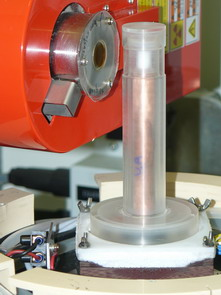
\includegraphics[width=4cm]{images/digitalSnow/YTEjpE}
\end{wrapfigure}
%
micro-structures de neige acquises en utilisant des techniques de tomographie à
rayons X (image de droite\footnote{Crédit image : laboratoires 3SR / MétéoFrance / CEN - CNRM GAME}). En effet,
lors d'une chute de neige, les cristaux de neige s'accumulent sur le sol et
forment progressivement un milieu poreux complexe constitué d'air, de vapeur
d'eau, de glace et parfois d'eau liquide. La quantité de ces composants et leur
arrangement géométrique à l'échelle granulaire (micro-structure de neige) se
transforme avec le temps en fonction des paramètres physiques de
l'environnement. Cette transformation est appelée la métamorphose, et peut être
décomposée en deux types : la métamorphose de la « neige humide » provoqué par
la présence d'eau liquide, la métamorphose de la « neige sèche » (métamorphose
d'isothermie et métamorphose du gradient de température).

\begin{figure}[ht]
    \begin{center}
    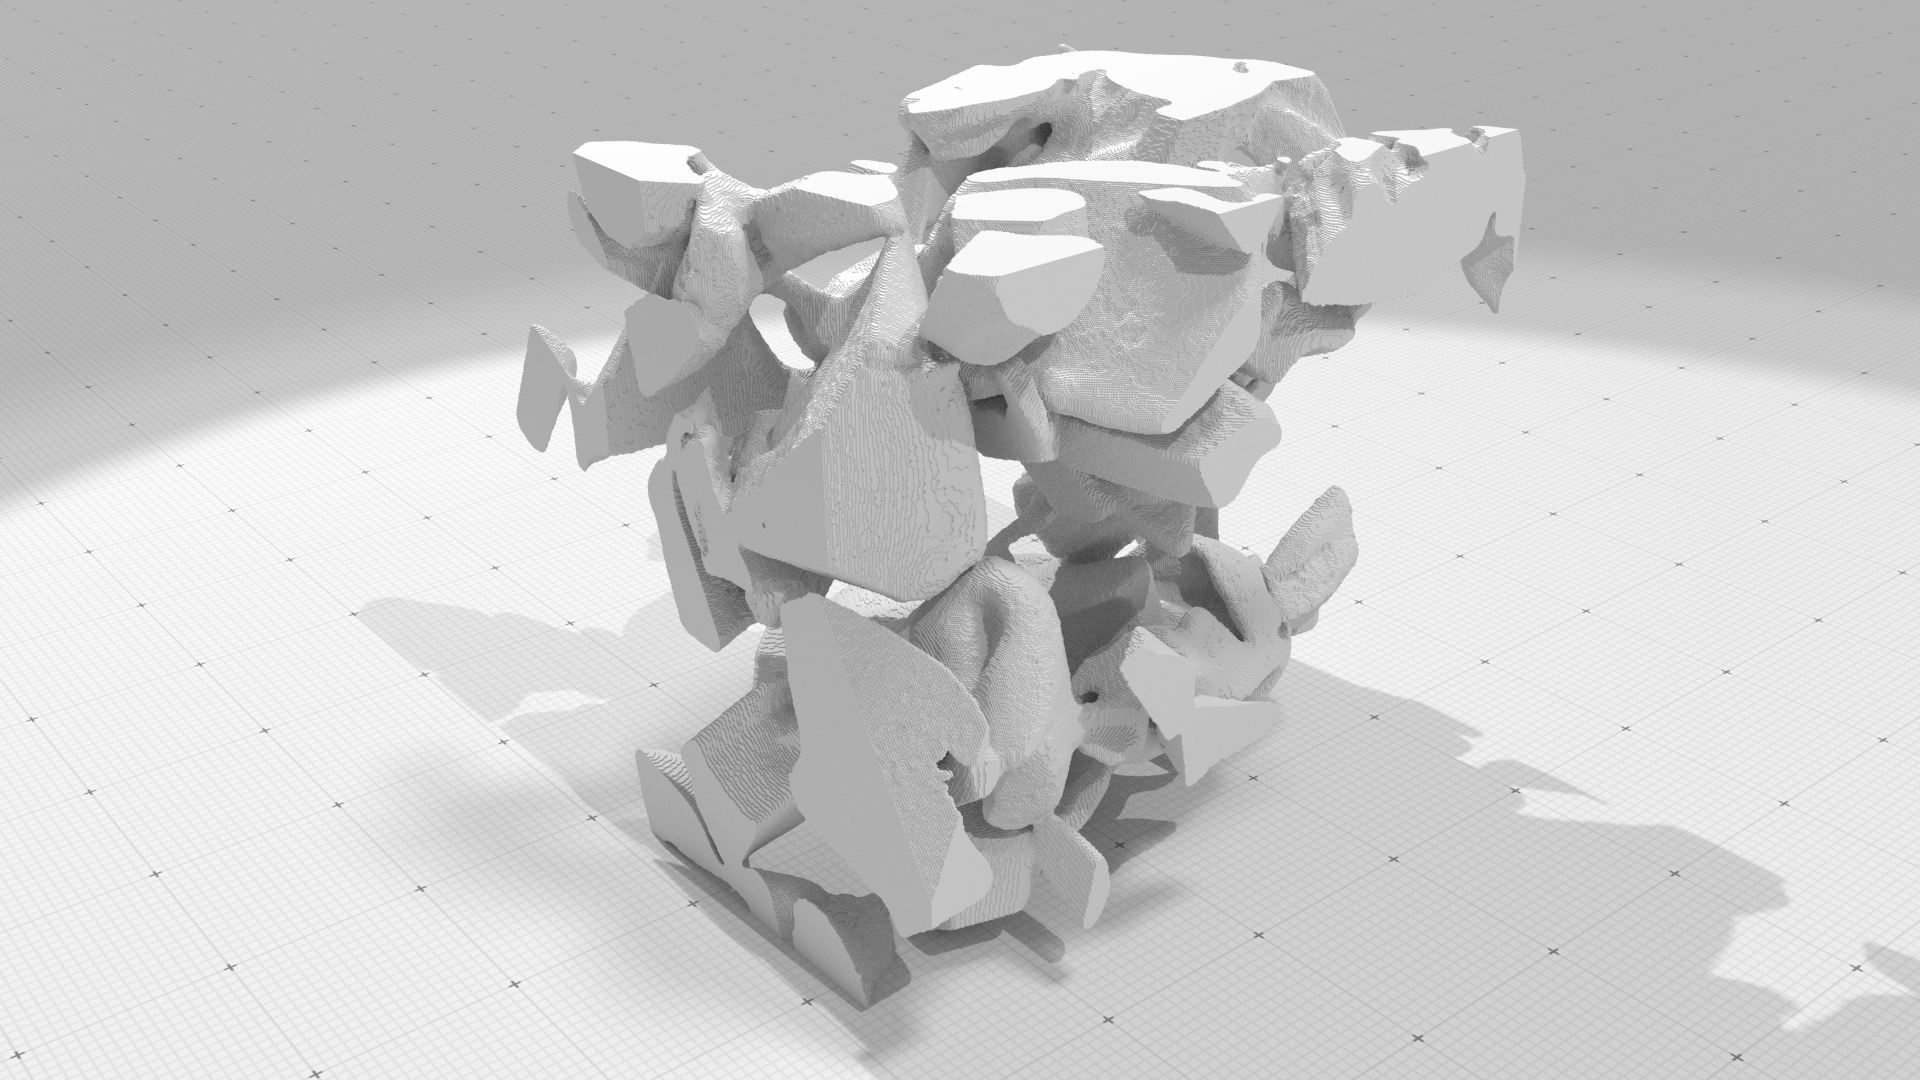
\includegraphics[trim={17cm 0 13cm 0},clip,width=6.7cm]{images/digitalSnow/SnowE2_DigitalData}
    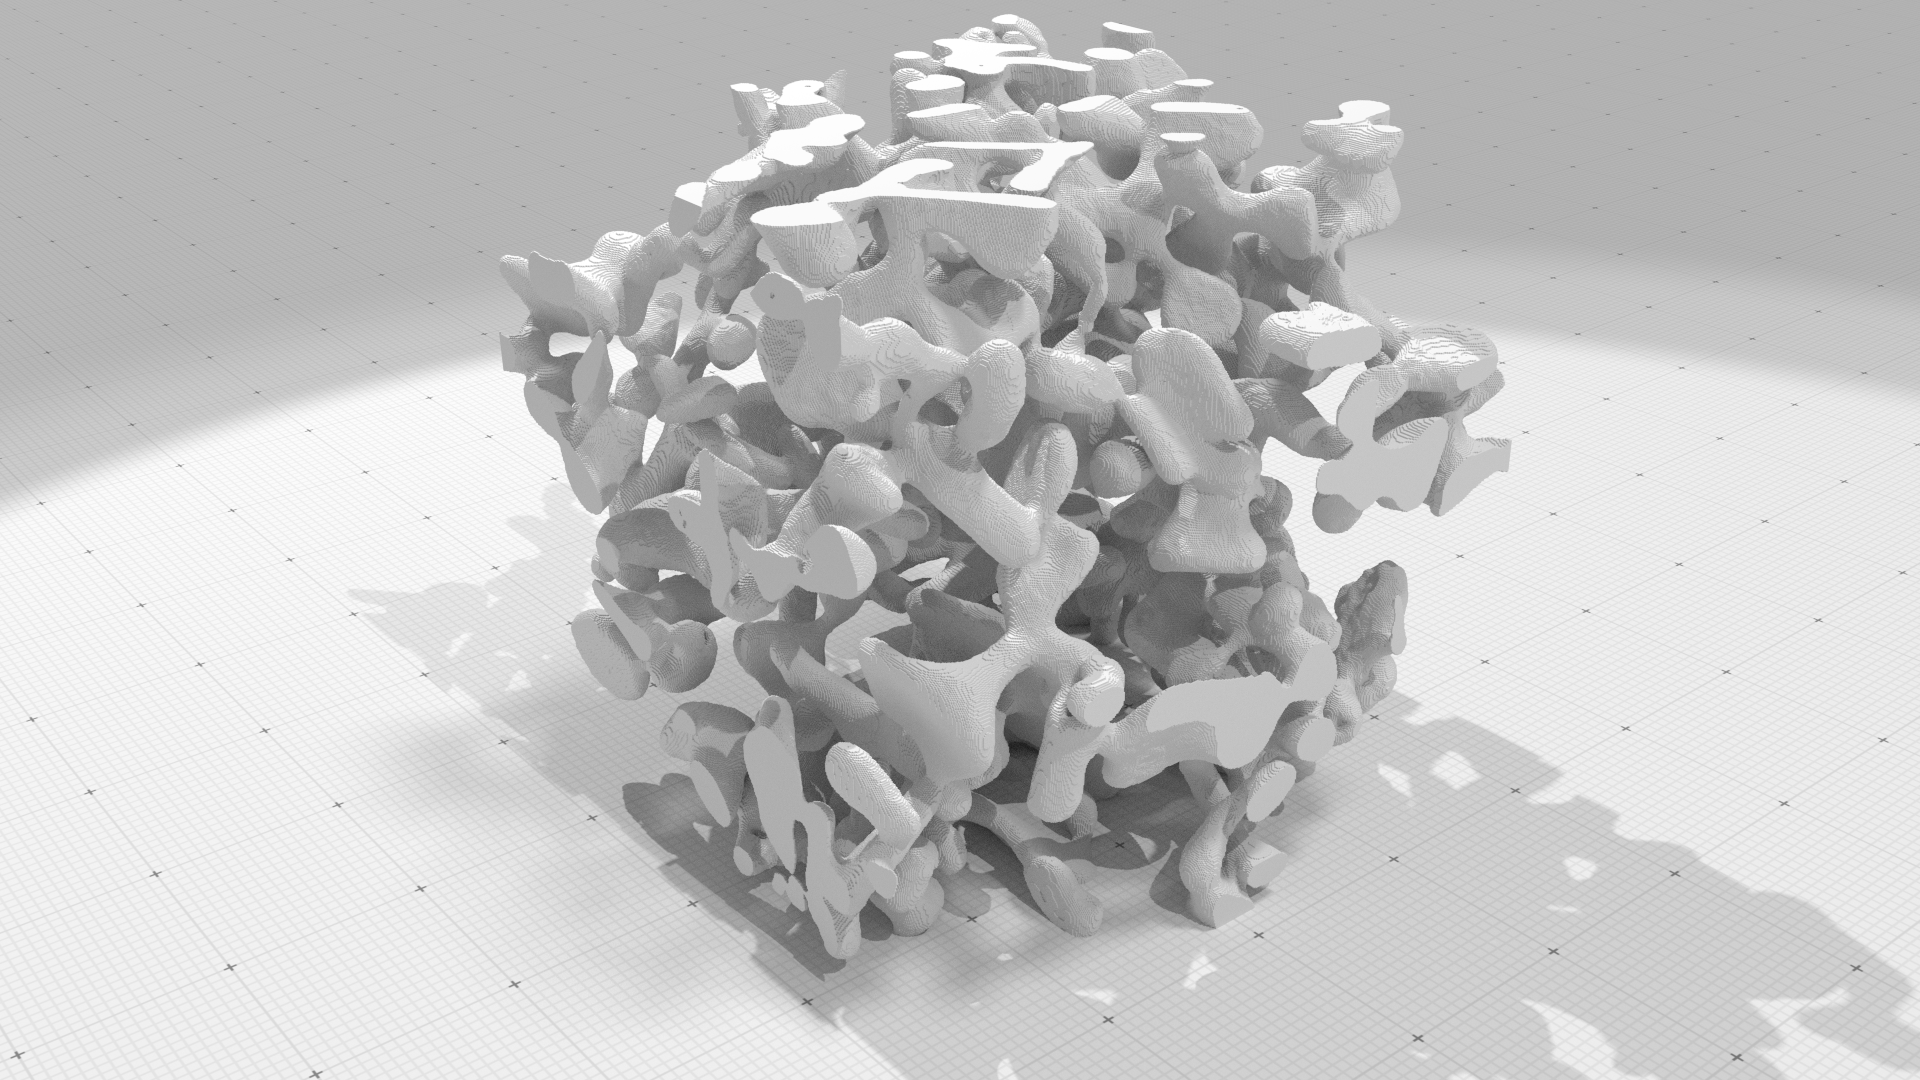
\includegraphics[trim={17cm 0 13cm 0},clip,width=6.7cm]{images/digitalSnow/SnowI08_DigitalData}\\
    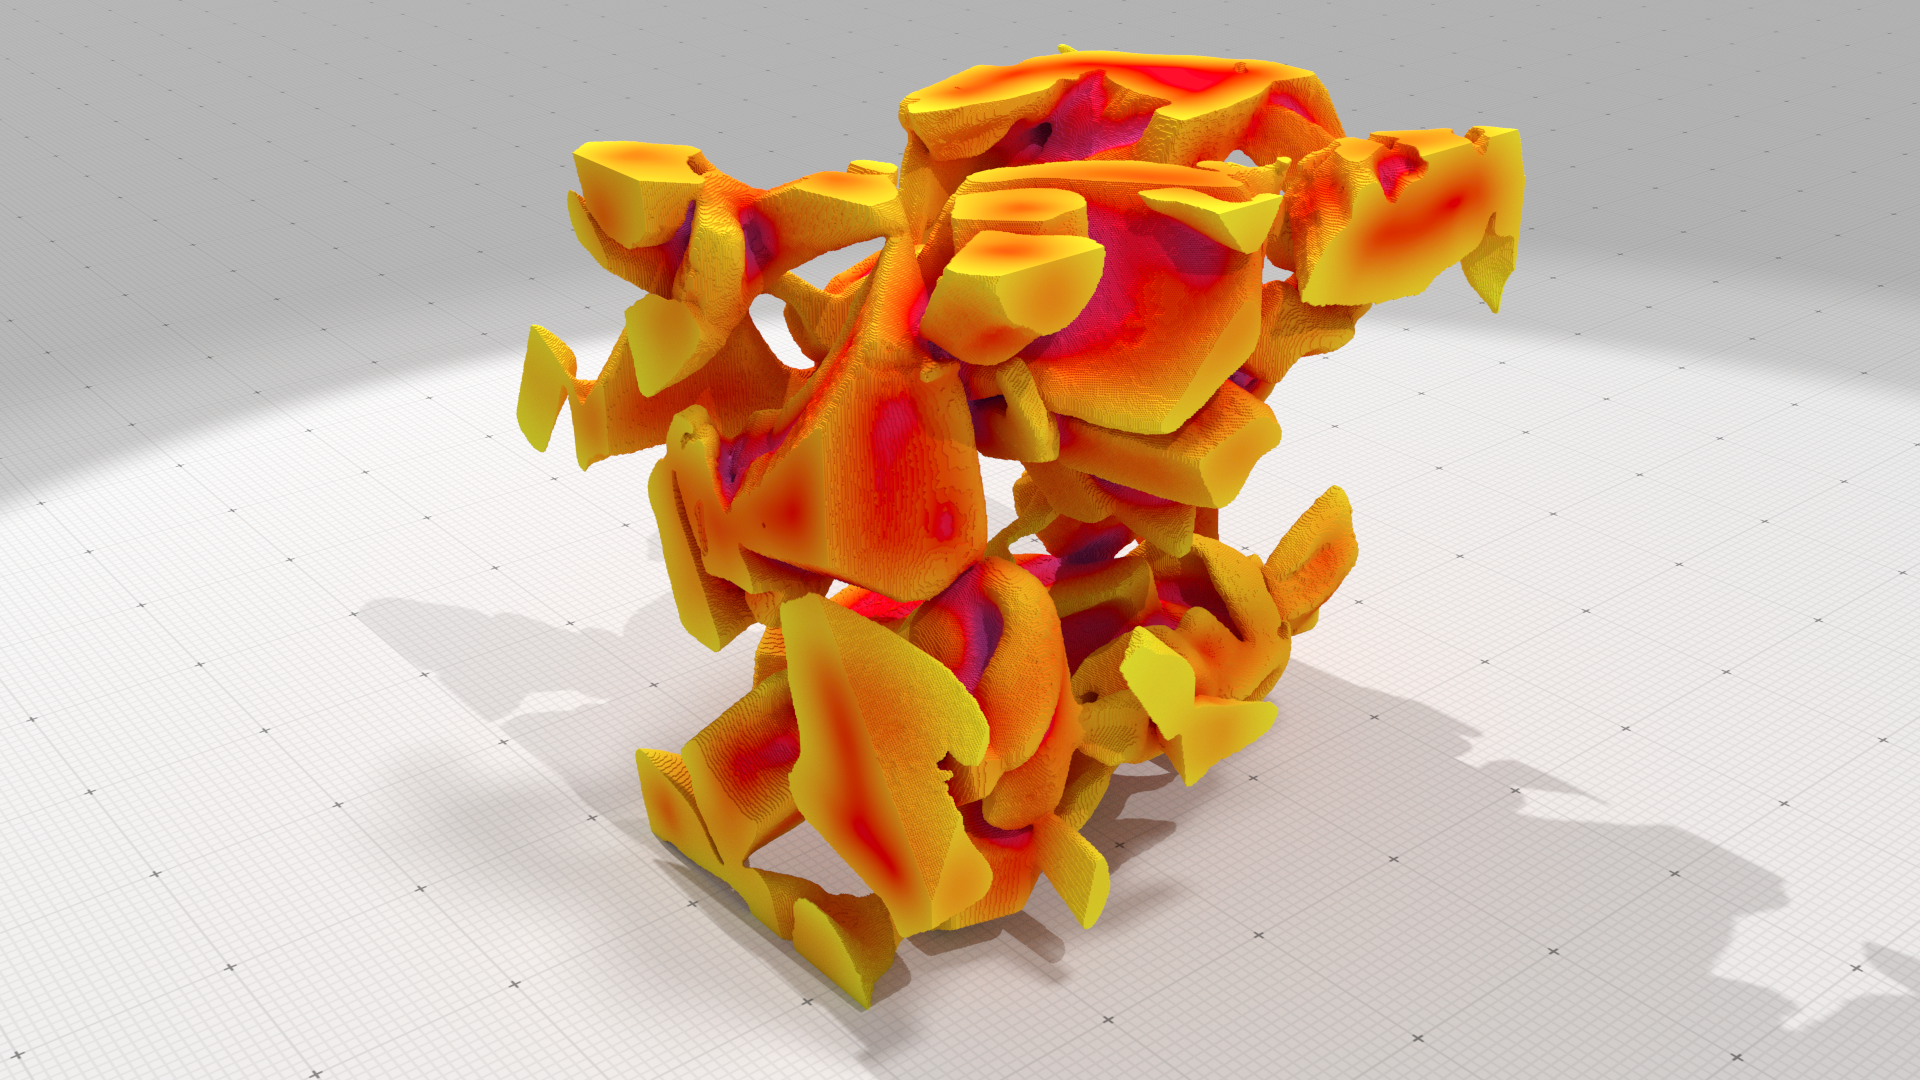
\includegraphics[trim={17cm 0 13cm 0},clip,width=6.7cm]{images/digitalSnow/snowE2mean_0001}
    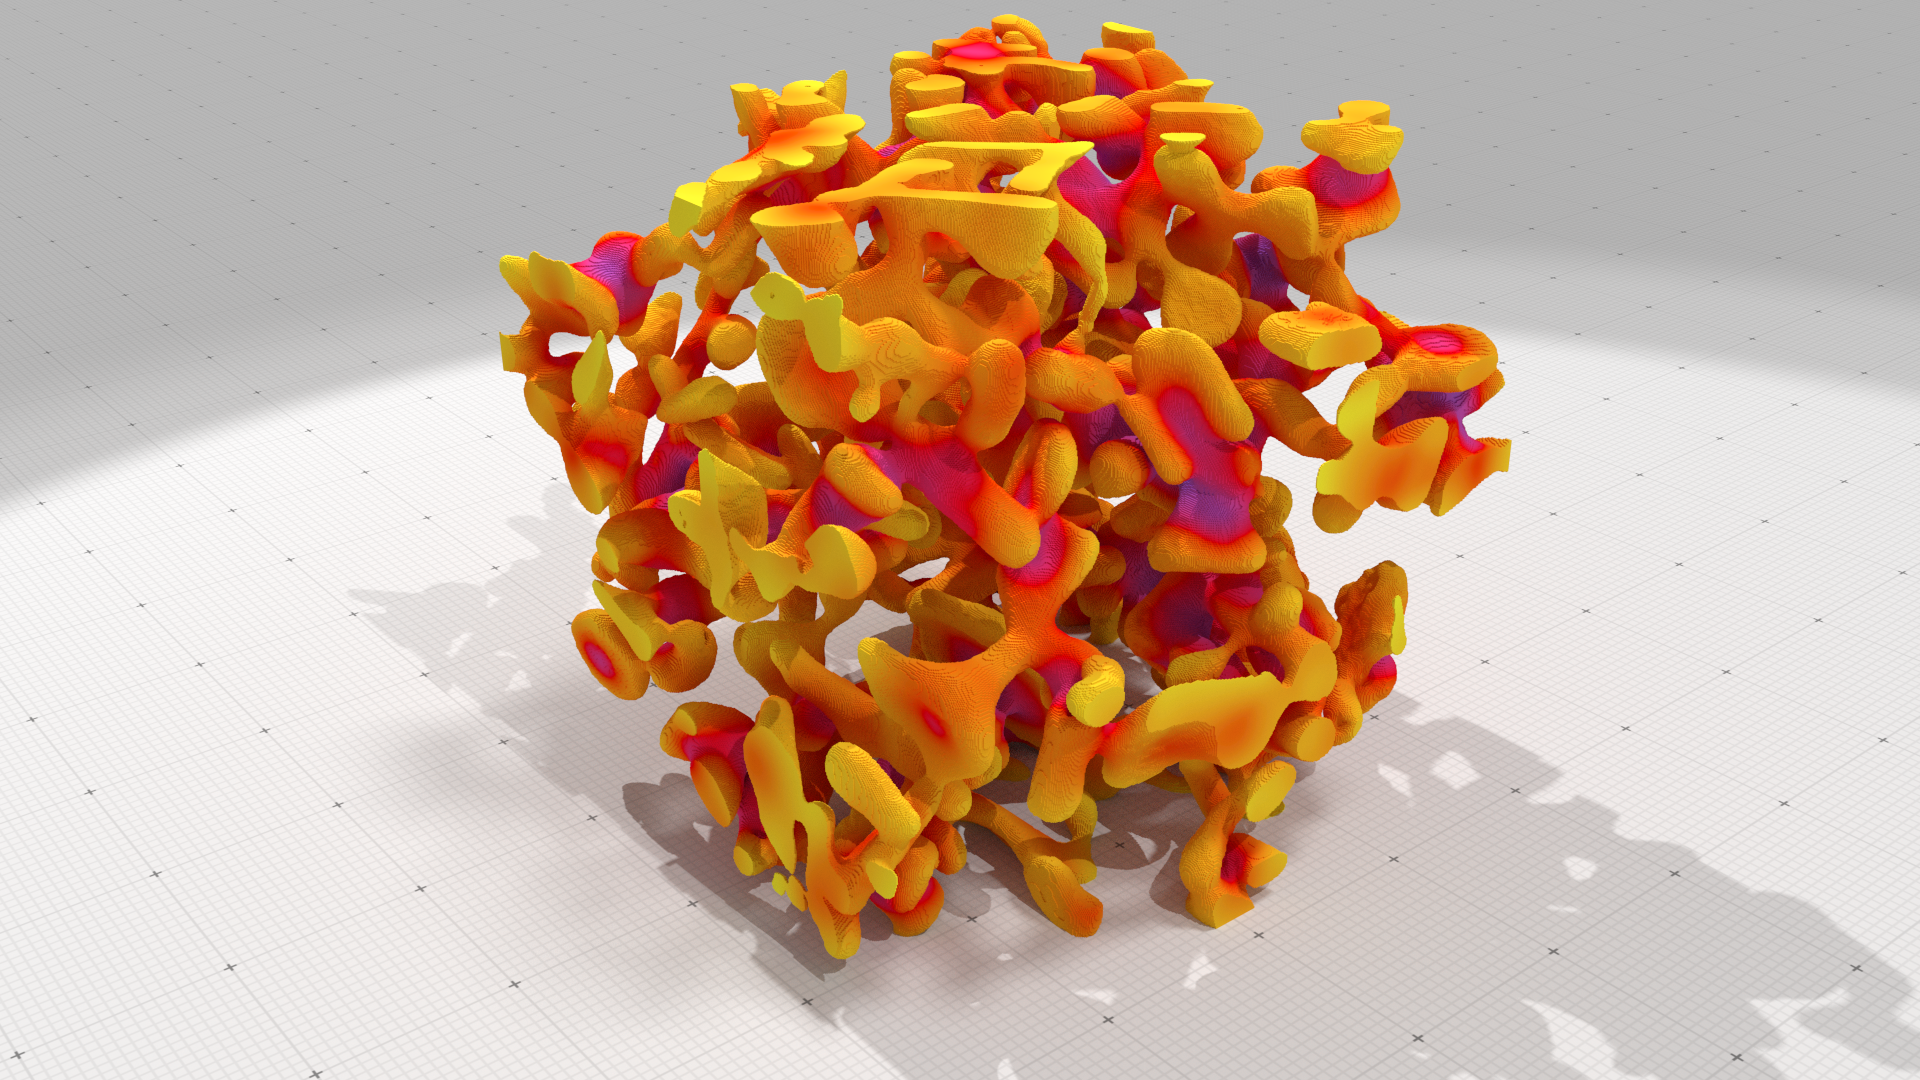
\includegraphics[trim={17cm 0 13cm 0},clip,width=6.7cm]{images/digitalSnow/snowI08mean_0001}
    \end{center}
    \caption{\emph{Première ligne :} Micro-structures de neige.
						 \emph{Seconde ligne :} Courbure moyenne sur ces échantillons de neige. La valeur de courbure va du bleu au jaune.
						 \label{fig:digitalSnow-curv}}
\end{figure}

\begin{figure}[ht]
    \begin{center}
    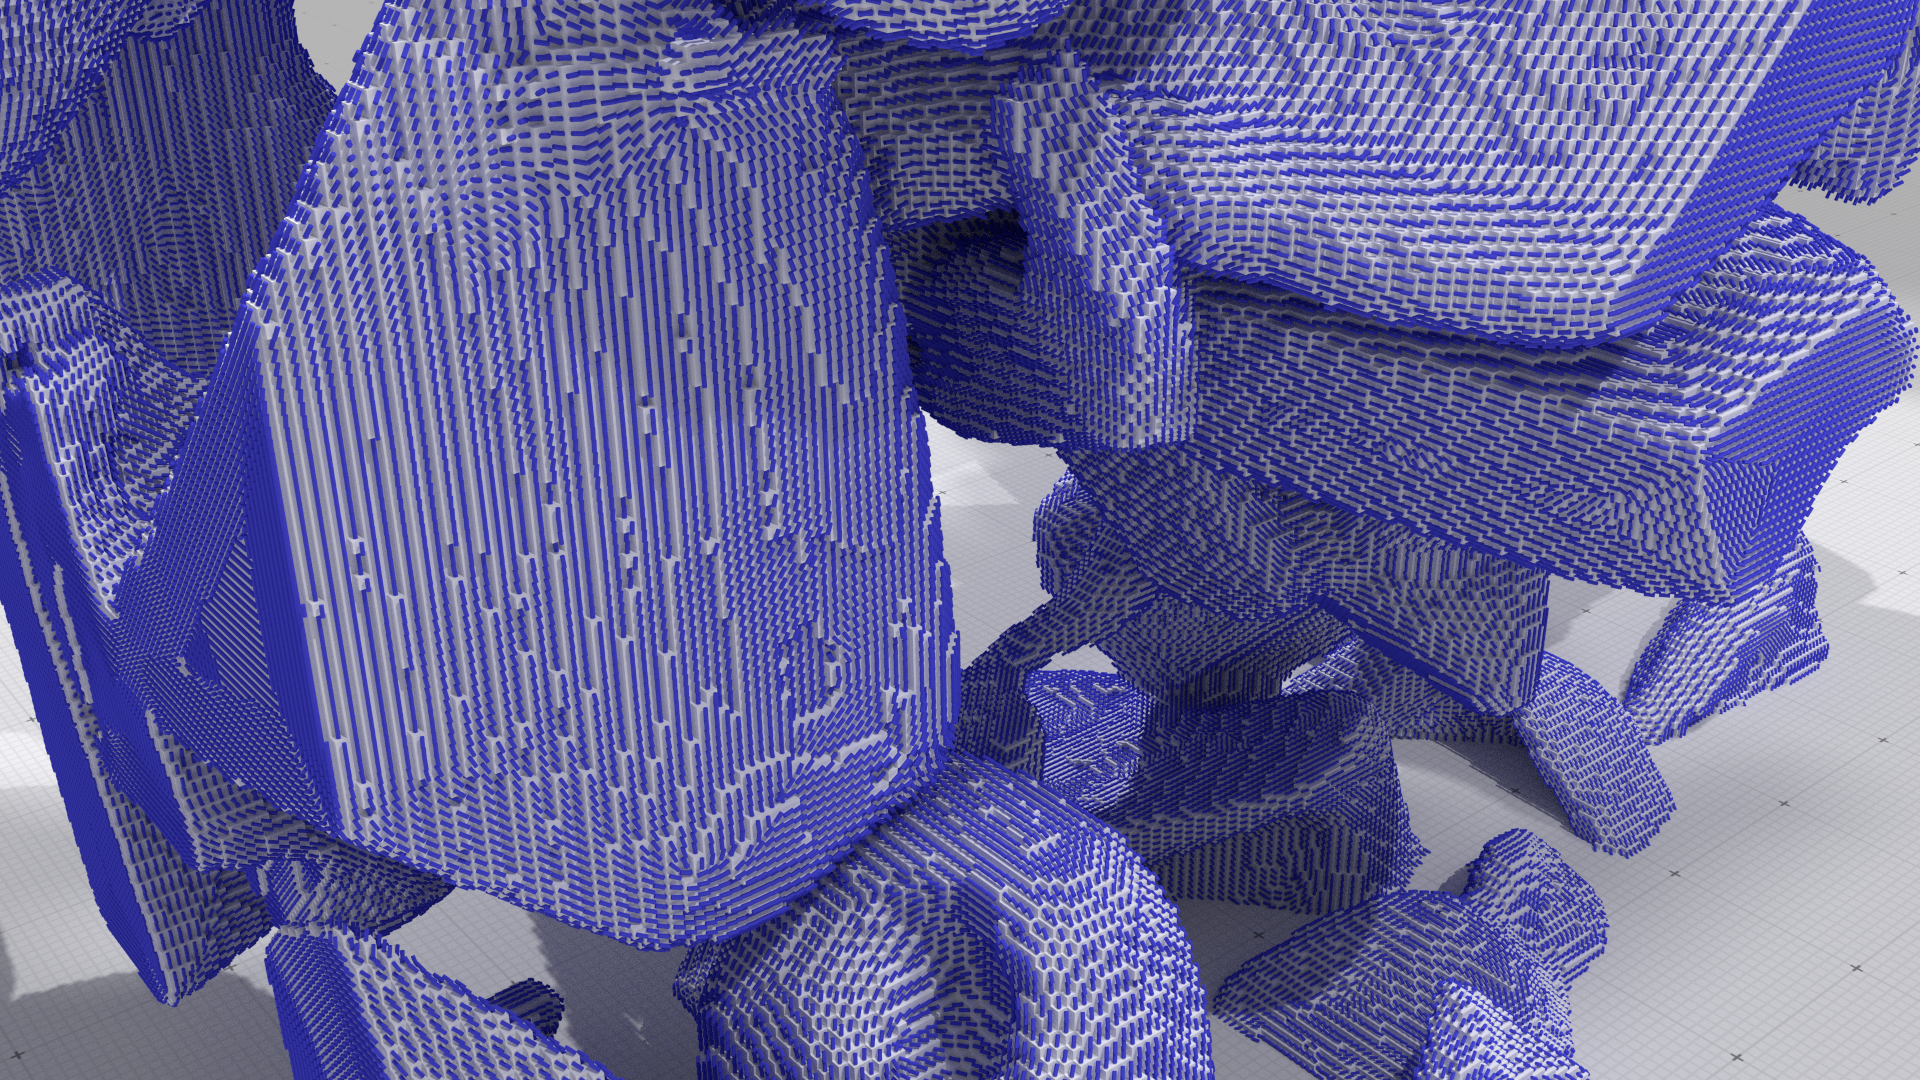
\includegraphics[trim={17cm 0 13cm 0},clip,width=6.7cm]{images/digitalSnow/E2bis-prindir-bleu}
		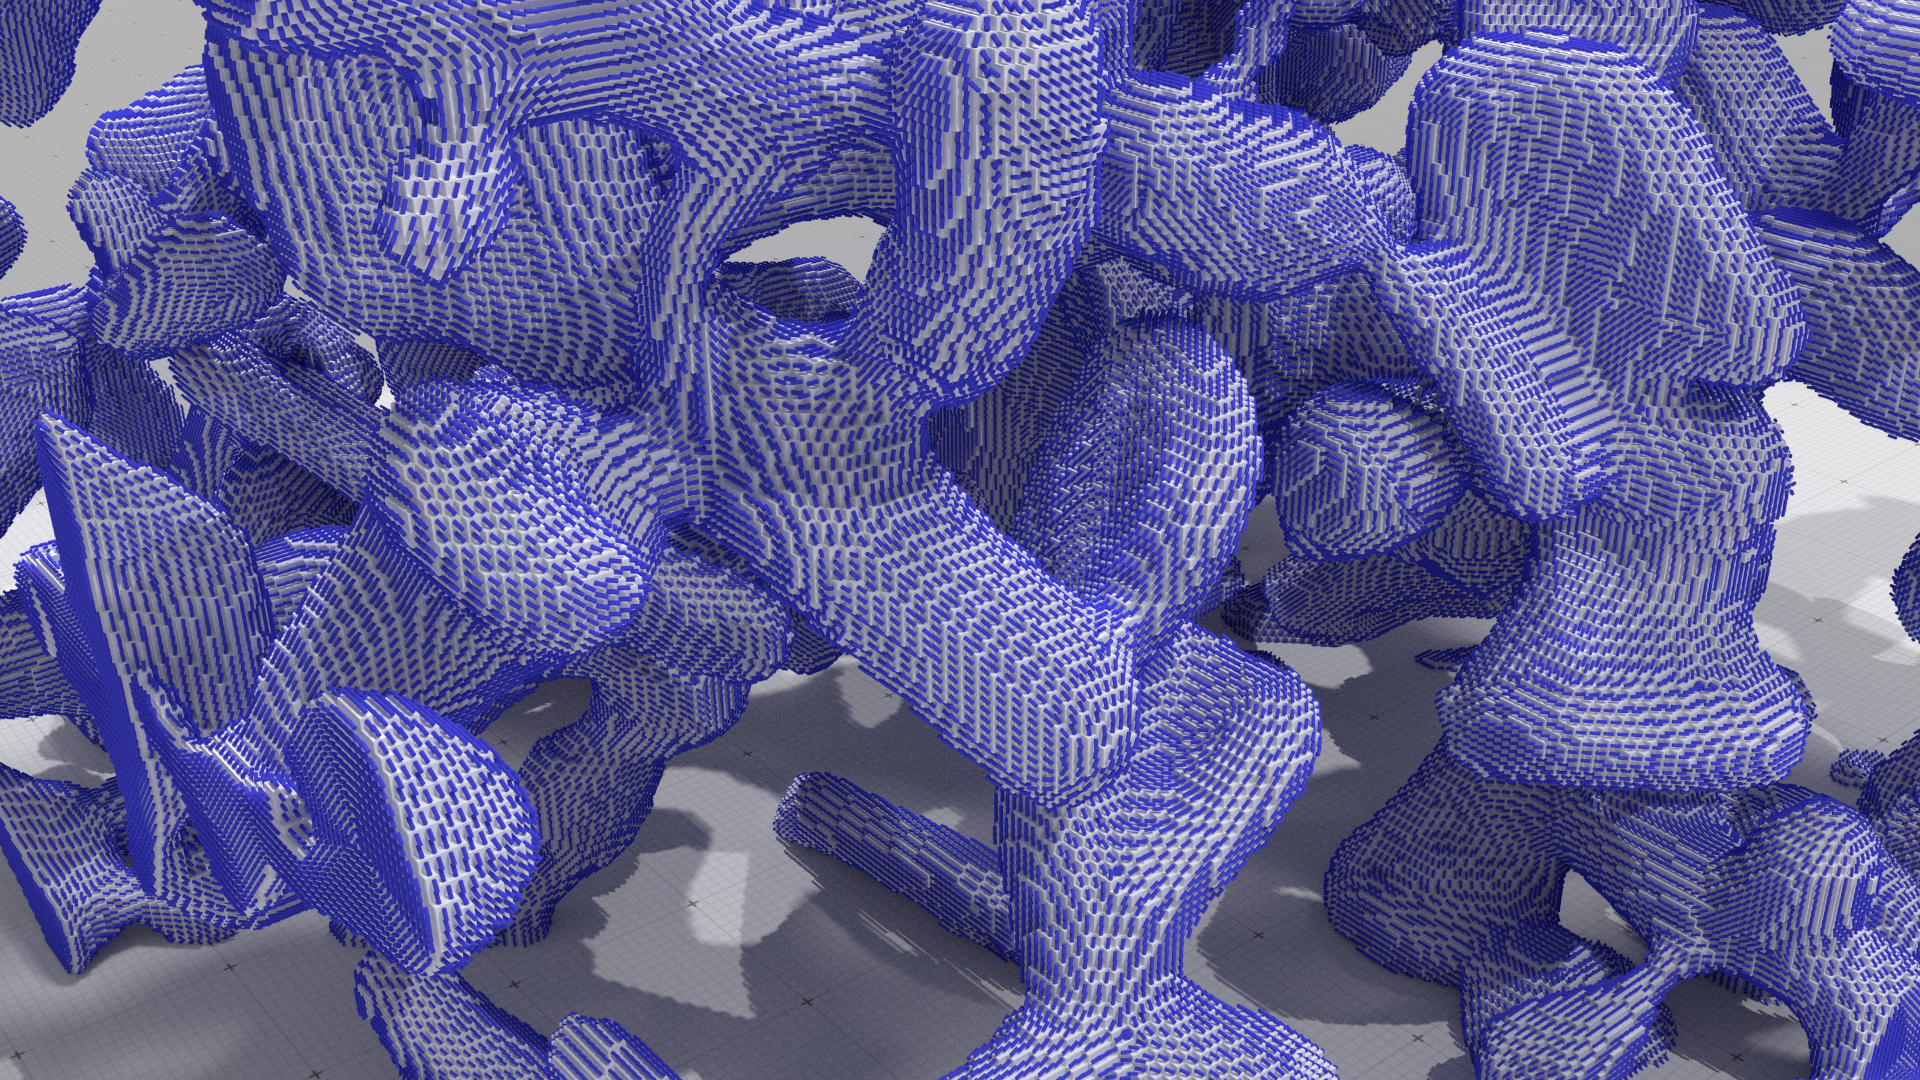
\includegraphics[trim={17cm 0 13cm 0},clip,width=6.7cm]{images/digitalSnow/I08prindir}\\
		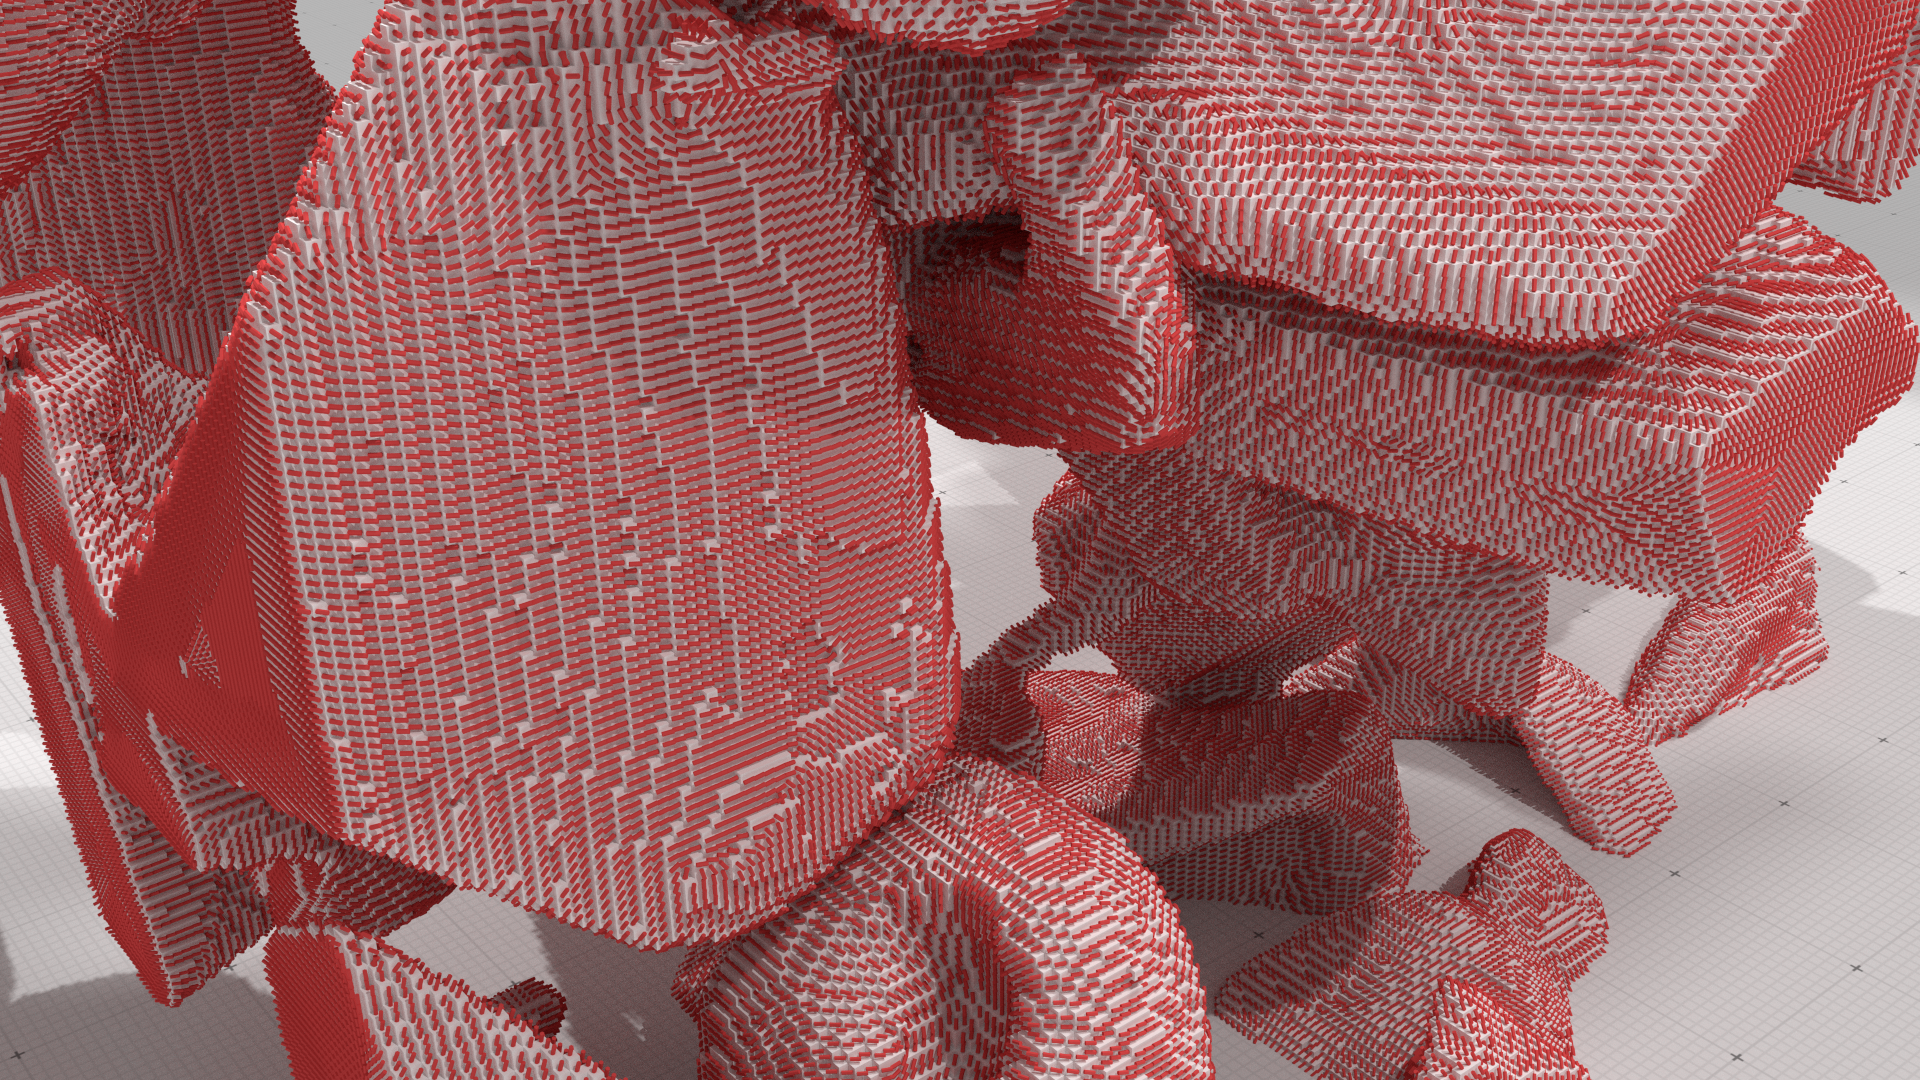
\includegraphics[trim={17cm 0 13cm 0},clip,width=6.7cm]{images/digitalSnow/E2bis-prindir-rouge}
    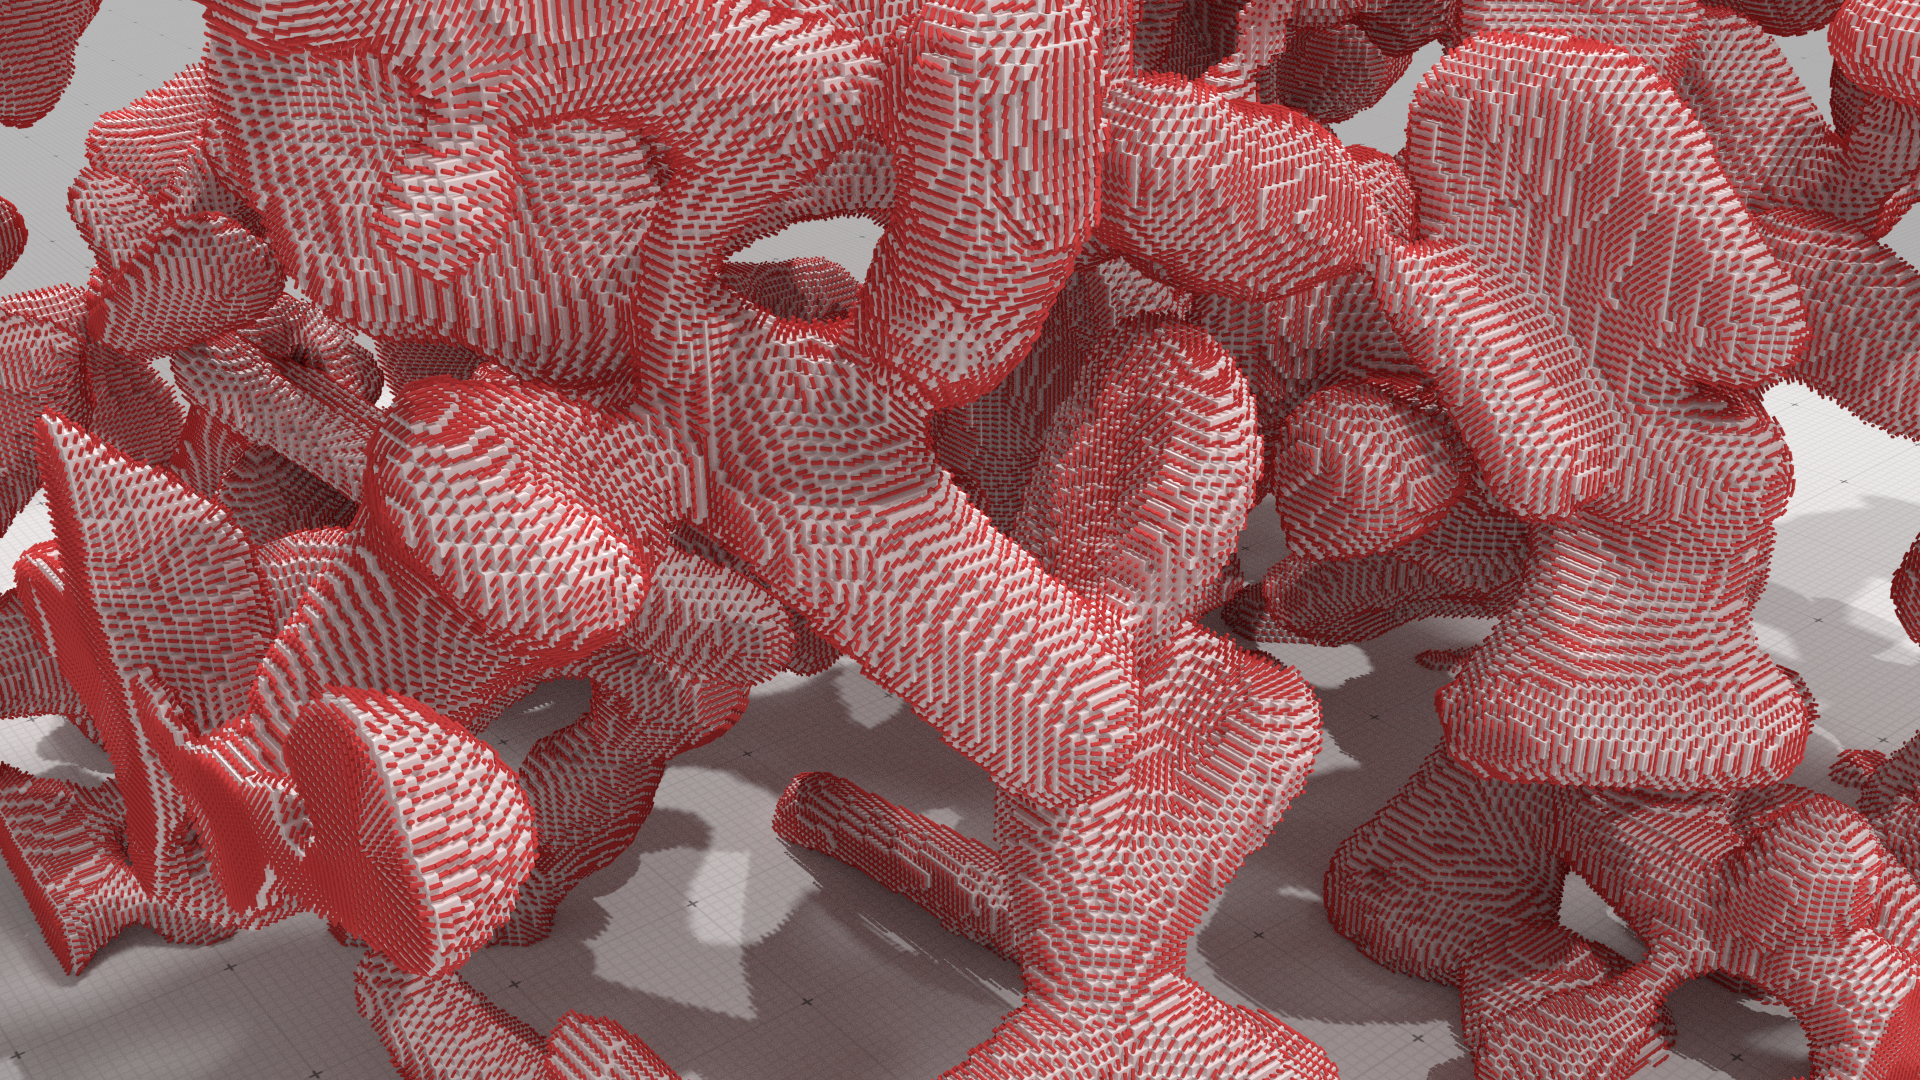
\includegraphics[trim={17cm 0 13cm 0},clip,width=6.7cm]{images/digitalSnow/I08prindir2}
    \end{center}
		%
    \caption{Zoom sur les premières directions principales de courbure
    (\emph{première ligne}) et secondes directions princpales de courbure
    (\emph{seconde ligne}) sur des échantillons de neige.
    \label{fig:digitalSnow-princdir}}
		%
\end{figure}

\begin{figure}[ht]{
    \begin{center}
    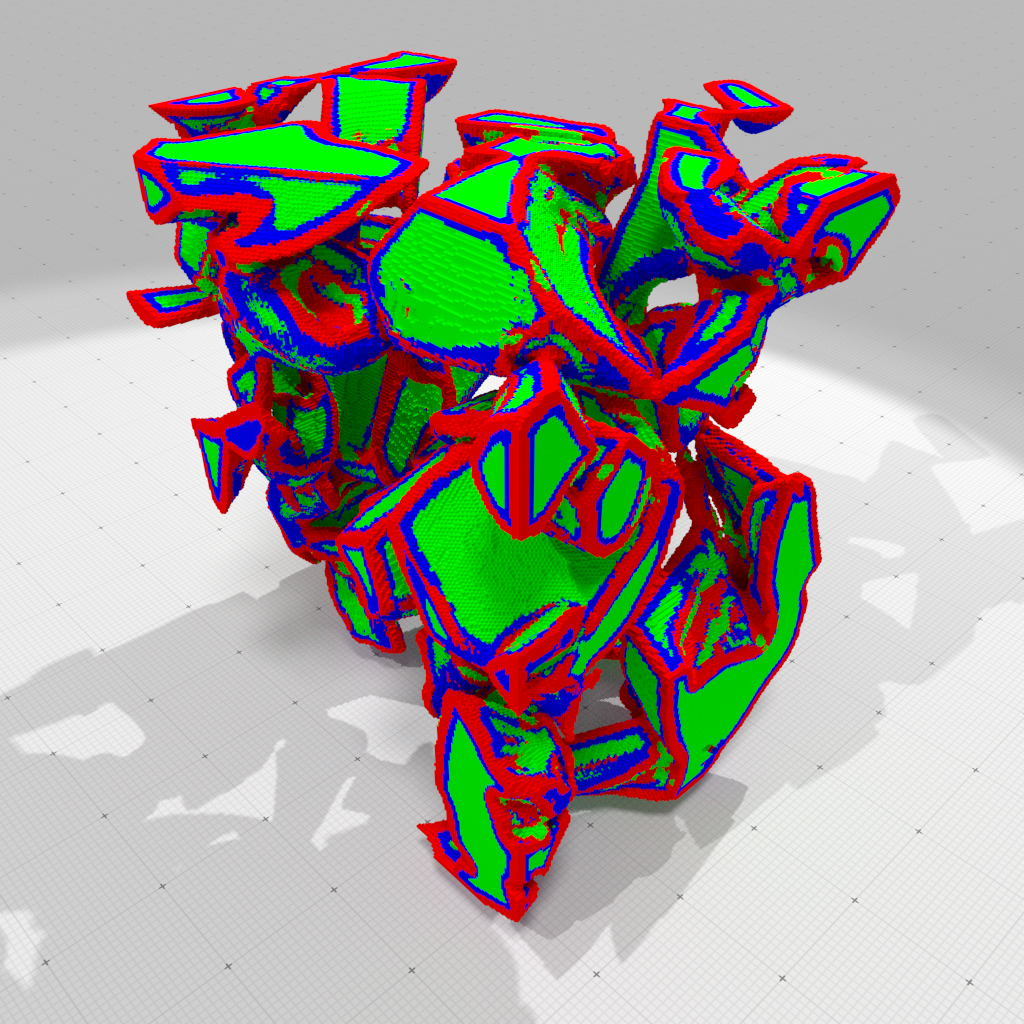
\includegraphics[width=6.7cm]{images/digitalSnow/Snow_E2bis_II_scale}
    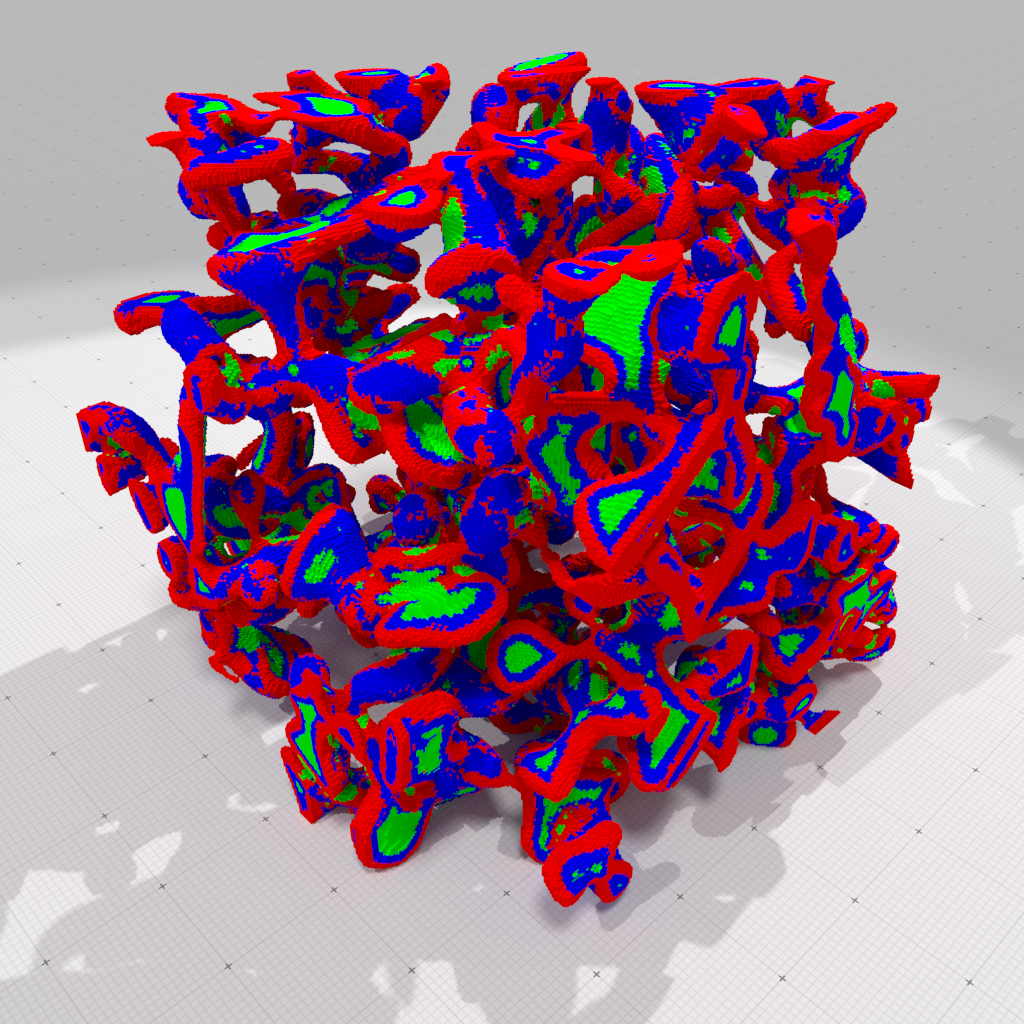
\includegraphics[width=6.7cm]{images/digitalSnow/Snow_I08_II_scale}\\
    \end{center}}
    \caption{Détection de singularités (\emph{en rouge}), de parties $C^3$ (\emph{en bleu}) et de parties à courbure nulle (\emph{en vert}) sur les échantillons de neige.
      \label{fig:digitalSnow-sing}}
\end{figure}

Dans des conditions polaires ou montagneuses, ces effets sont suivis par des
contraintes mécaniques comme le compactage de la neige sous l'effet du poids des
couches supérieures de neige. En particulier, notre travail se concentre sur le
développement de modèles numériques 3D à partir d'images pour simuler
l'évolution de la forme de la microstructure de la neige au cours de son
métamorphisme. Le calcul de courbure moyenne sur les volumes digitaux
(\RefFigure{fig:digitalSnow-curv}, en bas) permet tout d'abord de caractériser
le volume des grains de neige. En l'absence de gradient de température dans le
manteau neigeux, les grains grossissent et s'arrondissent lentement,
principalement guidé par un flot de courbure moyenne sur l'interface (Effet de
Kelvin). Cependant, en présence d'un gradient de température, les cristaux
croissent suivant leurs axes cristallographiques privilégiés et forment des
facettes. Nous pouvons également détecter ces facettes grâces à l'estimateur de
singularité dont nous avons décrit dans ce chapitre. La
\RefFigure{fig:digitalSnow-sing} montre deux captures de microstructures de
neige à différents moments. Il est alors immédiat que les grains de neige de
gauche présentent plus de facettes que ceux de droite. De plus, l'estimation de
la courbure permet de simuler certains métamorphoses de neige : les zones
convexes ont tendance à se sublimer tandis que la vapeur se condense dans les
zones concaves. Notre rôle était d'apporter des estimateurs de courbure et de
directions principales de courbure (\RefFigure{fig:digitalSnow-princdir})
fiables (c'est à dire avec des preuves de convergence), ce que nous avons fait
avec les estimateurs décrits dans le \RefChapitre{sec:estimators}. Ces
estimateurs sont actuellement utilisés et répondent aux attentes des partenaires
du projet \digitalSnow, tout en étant robustes au bruit lié à l'acquisition par
le tomographe à rayons X. Nous avons également proposé l'estimation de
singularités permettant de détecter les facettes des grains de neige (voir le
\RefSection{sec:applications:feature}).

\section{Implémentations dans DGtal}%
\label{sec:applications:dgtal}
%
Nous avons implémenté tous les estimateurs présentés dans ce manuscrit dans
\DGtal \cite{DGtal}. Le projet \DGtal (\anglais{Digital Geometry Tools and Algorithms},
\url{http://dgtal.org}) est une bibliothèque collaborative open-source écrite en
\textsc{C++} proposant des structures de données, algorithmes et outils
génériques, fiables et efficaces pour la \DigitalGeometry. Son code source est
disponible sur GitHub (\url{https://github.com/DGtal-team/DGtal/}).

Un des objectifs de \DGtal est de centraliser toutes les techniques dédiées à la
géométrie digitale (et domaines proches comme la topologie digitale, le
traitement d'image, etc.) dans un même lieu, facilitant ainsi leur usage. Un des
exemples le plus représentatif est la branche « estimateurs » de \DGtal :
celle-ci comptabilise plusieurs estimateurs de quantités intégrales comme
les tangentes, les normales, le périmètre, et dans notre cas la courbure. Dans
notre processus de convergence asymptotique, nous avons besoin de discrétiser à
plusieurs échelles des formes euclidiennes auxquelles nous savons en tout point
la valeur de la quantité intégrales que nous estimons. Encore une fois,
\DGtal nous simplifie la tâche en nous proposant de générer des formes
paramétriques et implicites de dimension 2 et 3 que nous pouvons discrétiser à
plusieurs échelles, ainsi que la possibilité de charger et exporter des objets.
Ensuite, \DGtalTools (le projet annexe de \DGtal proposant des applications des
algorithmes présents dans \DGtal) possède une plate-forme de comparaison
d'estimateurs permettant d'exporter les résultats : \texttt{2dLocalEstimators}
et \texttt{3dLocalEstimators}. C'est grâce à ces outils que nous avons généré
toutes les courbes de comparaison de ce document.

Le modèle topologique utilisé dans \DGtal est celui de l'espace de
Khalimsky\footnote{Documentation du paquet « Topologie » :
\url{http://dgtal.org/doc/stable/packageTopology.html}} (nous l'avons défini
dans le \RefSection{sec:digitization}). Les cellules de Khalimsky sont définies
dans un domaine de Khalimsky, \cad une grille cubique de dimension $n$.
Plusieurs algorithmes d'extraction et de suivi de surface sont disponibles et
adaptés à cette topologie. Concrètement, \DGtal peut nous fournir un itérateur
de surfels de la surface nous permettant de la parcourir en profondeur ou en
largeur de manière optimale, \cad en évitant autant que possible les
déplacements non connexes. Cette propriété est très importante dans notre cas si
nous voulons optimiser la complexité de notre estimation de la courbure. Comme
nous l'avons dit dans le \RefSection{sec:complexite}, nous pouvons réduire le
calcul de l'intégration volumique de la sphère avec la surface de l'objet en
utilisant les informations de l'itération précédente. En effet, comme le montre
la \RefFigure{fig:MovingKernel2D} en haut à gauche, si nous nous déplaçons à une
distance $\delta$ inférieure au rayon de la sphère, nous calculons à nouveau une
partie du résultat précédent. Afin d'éviter cette redondance de calcul, nous
pouvons pré-calculer des masques de déplacement pour toutes les voisins
$0$-adjacents à un point (à droite sur la \RefFigure{fig:MovingKernel2D}).
Ainsi, au lieu de dénombrer le nombre de points digitaux sur la sphère digitale
entière, nous pouvons récupérer le dénombrement de l'itération (hachurée),
retirer la partie qui n'est plus partagée avec la nouvelle position (en orange),
et ajouter celle qui est nouvelle (en vert).
Dans le pire des cas (déplacement non $0$-adjacent), l'estimateur utilisera
l'intégralité du support pour le dénombrement de l'intersection de la sphère et
de l'objet, \cad qu'il n'y aura aucune optimisation. Comme nous l'avons dit
précédemment (\RefSection{sec:complexite}), le coût du calcul par élément de
surface peut être réduit de $O\left(\left(\frac{R}{h}\right)^d\right)$ (taille du support complet) à
$O\left(\left(\frac{R}{h}\right)^{d-1}\right)$. Pour être tout à fait juste, il faut également
rajouter le coût initial du premier calcul obligatoire sur le support entier, et
le coût supplémentaire au début pour pré-calculer les masques de déplacement,
mais ceux-ci sont négligeable. Par exemple, pour une taille de support 2D entier
de $\nombre{91893}$ éléments, l'optimisation construit de $8$ masques de
déplacements supplémentaires d'environ $\nombre{450}$ éléments.

\begin{figure}[th]
  \centerline{
  %\input[width=2.9cm]
  %width=2.9cm

\begin{tikzpicture}[x=0.28cm,y=0.28cm]
  % colors
  \definecolor{kGreen}{rgb}{0.0,0.59,0.0}
  \definecolor{kOrange}{rgb}{1.0,0.59,0.0}
  \definecolor{kGrey}{rgb}{0.33,0.33,0.33}
  % grids

  \node (px) at (5.5,6) {};
  \node (px2) at (6.5,6) {};
  \node (px3) at (7.5,5.9) {};

  \draw[draw,thick,fill,color=kOrange,nearly transparent] (px) circle (4);
  \draw[draw,thick,fill,color=kGreen,nearly transparent] (px2) circle (4);

  \draw[pattern=north west lines, pattern color=red] (5.5,10) arc (90:-90:4);
  \draw[pattern=north west lines, pattern color=red] (6.5,2) arc (270:90:4);

  \draw[draw,thick,color=kOrange] (px) circle (4);
  \draw[draw,thick,color=kGreen] (px2) circle (4);

  \draw[draw,thick,color=black,fill] (px) circle (0.1);
  \draw[draw,thick,color=black,fill] (px2) circle (0.1);
  \draw (px) node[above] {\scriptsize$\mathbf{x}$};
  \draw (px3) node[above] {\scriptsize$\mathbf{x} + \vec{\delta}$};

\end{tikzpicture}
%images/digitalSnow/MovingKernel_r}
  
\includegraphics[width=0.62cm,keepaspectratio=false]{images/misc/TransparentPixel}
  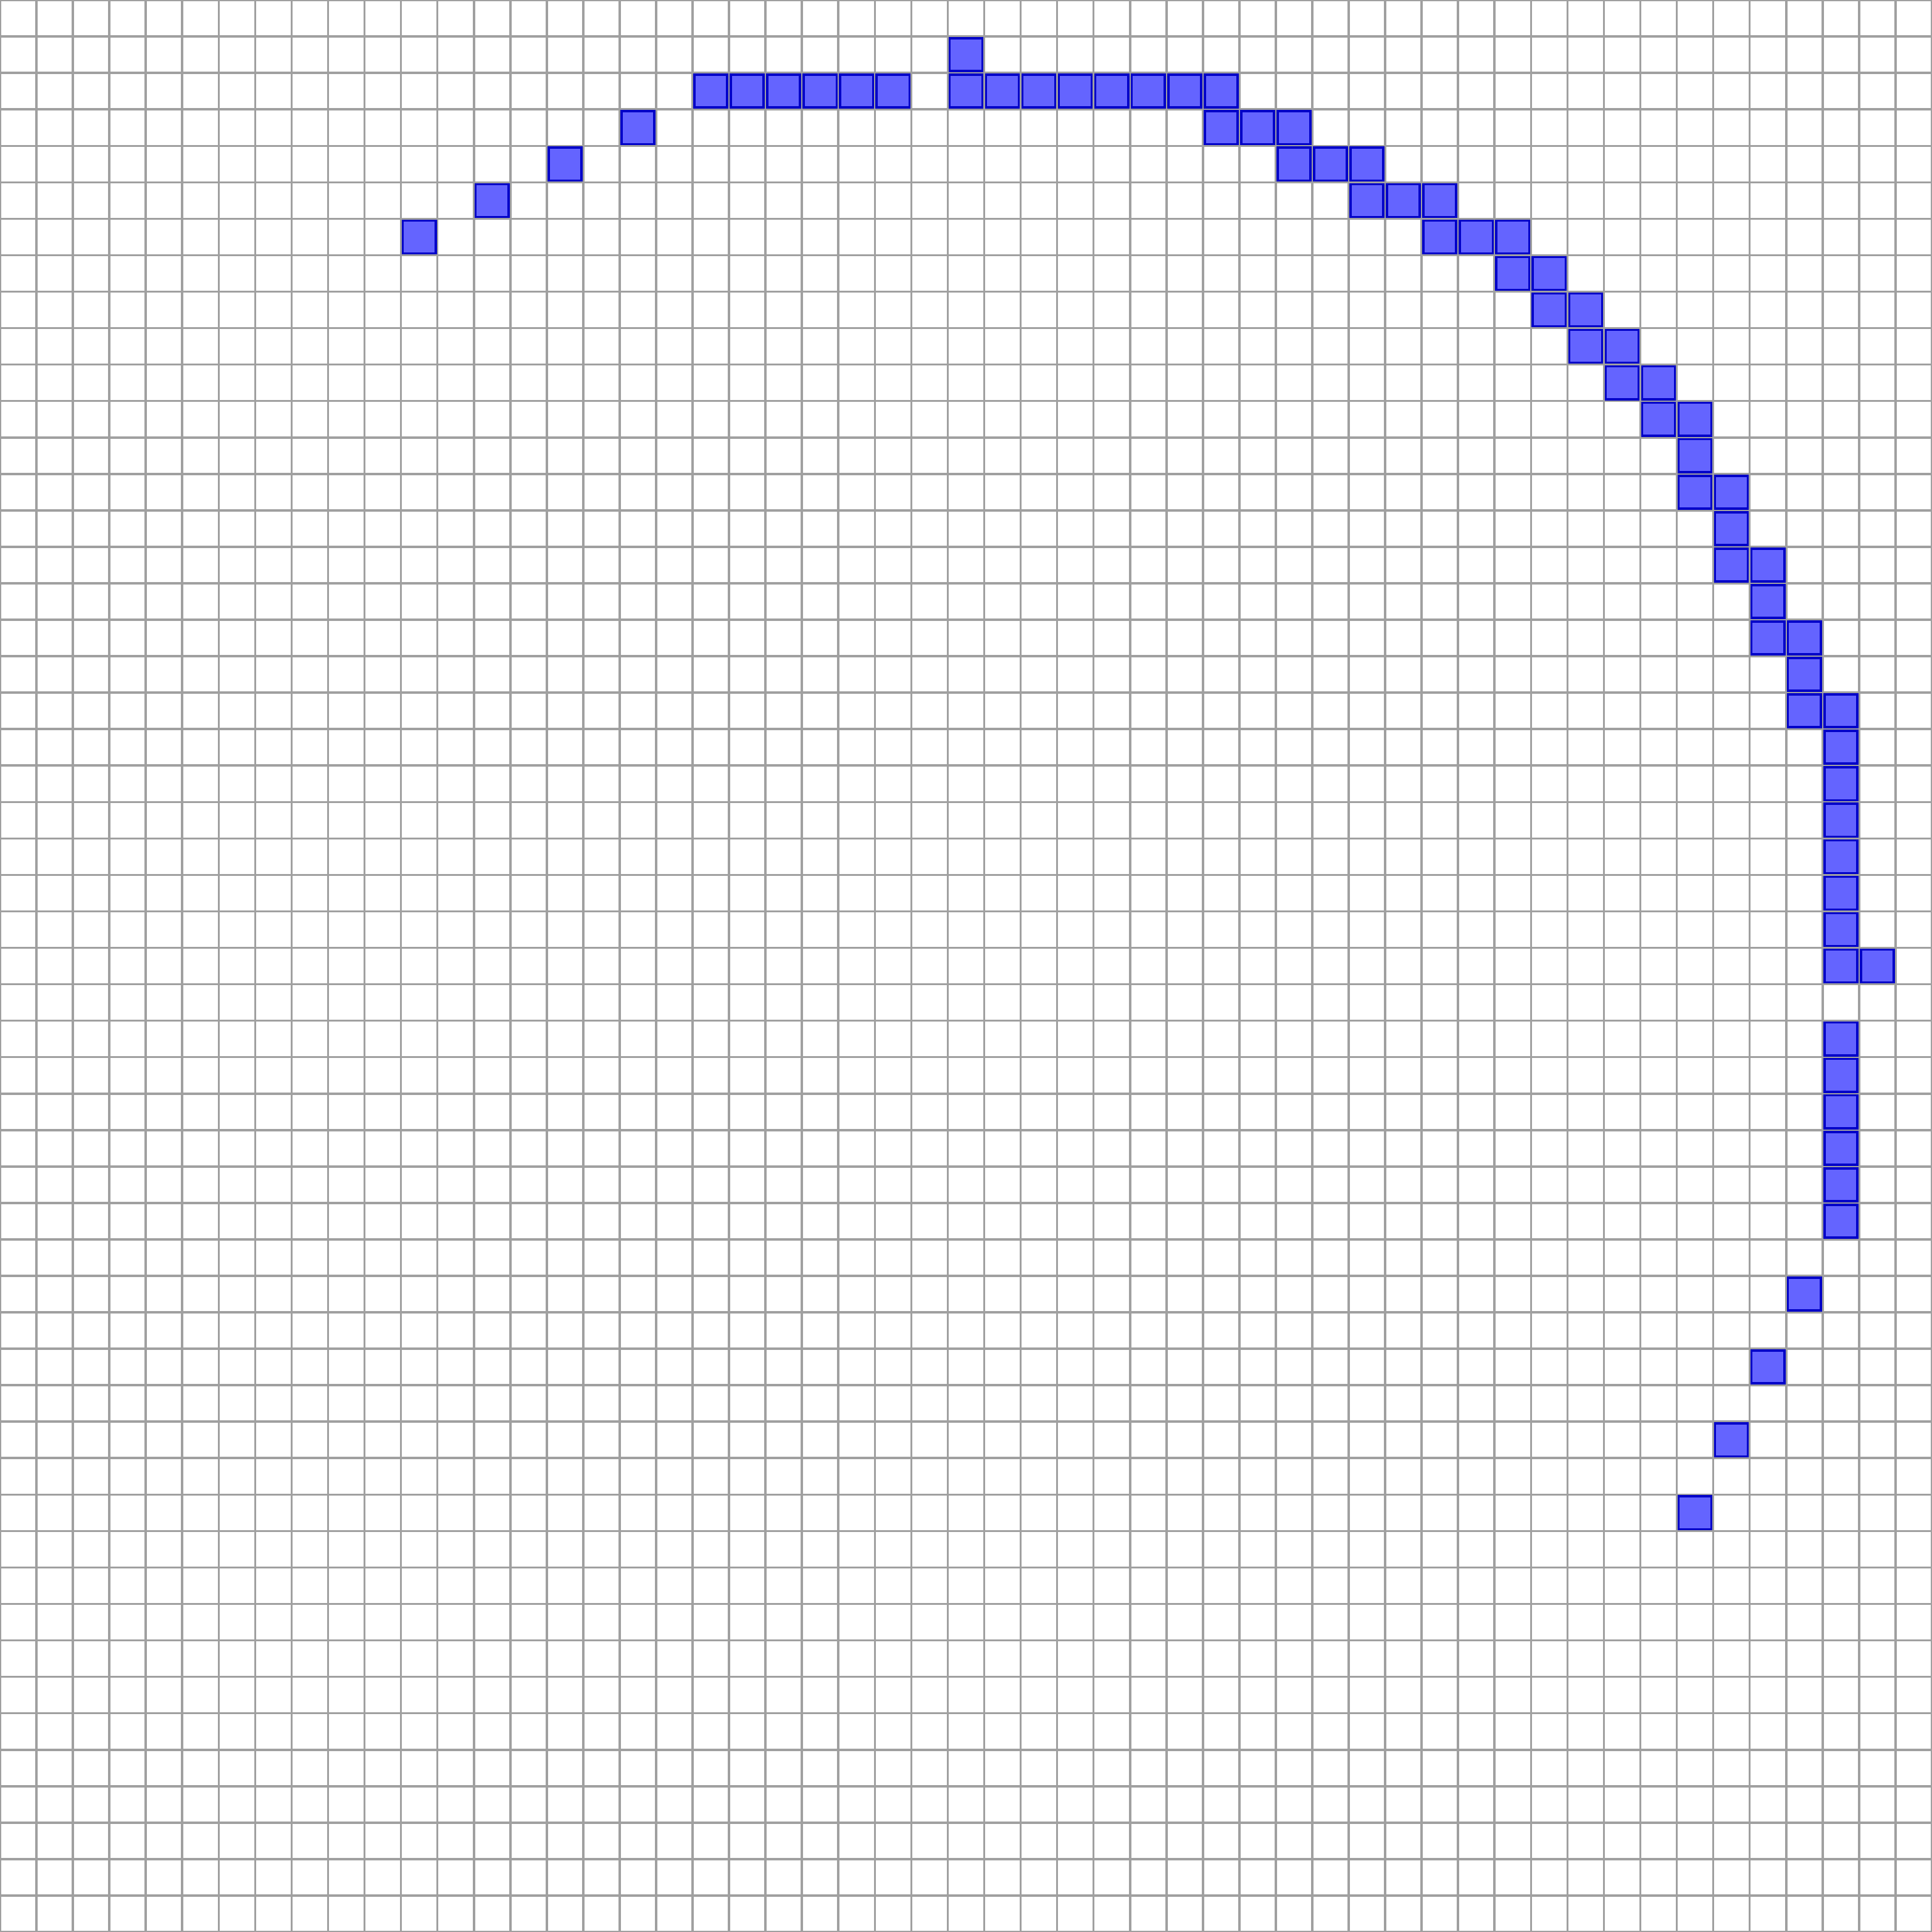
\includegraphics[width=2.5cm]{images/digitalSnow/testIntegralInvariantCurvatureEstimator-PartialMask0}
  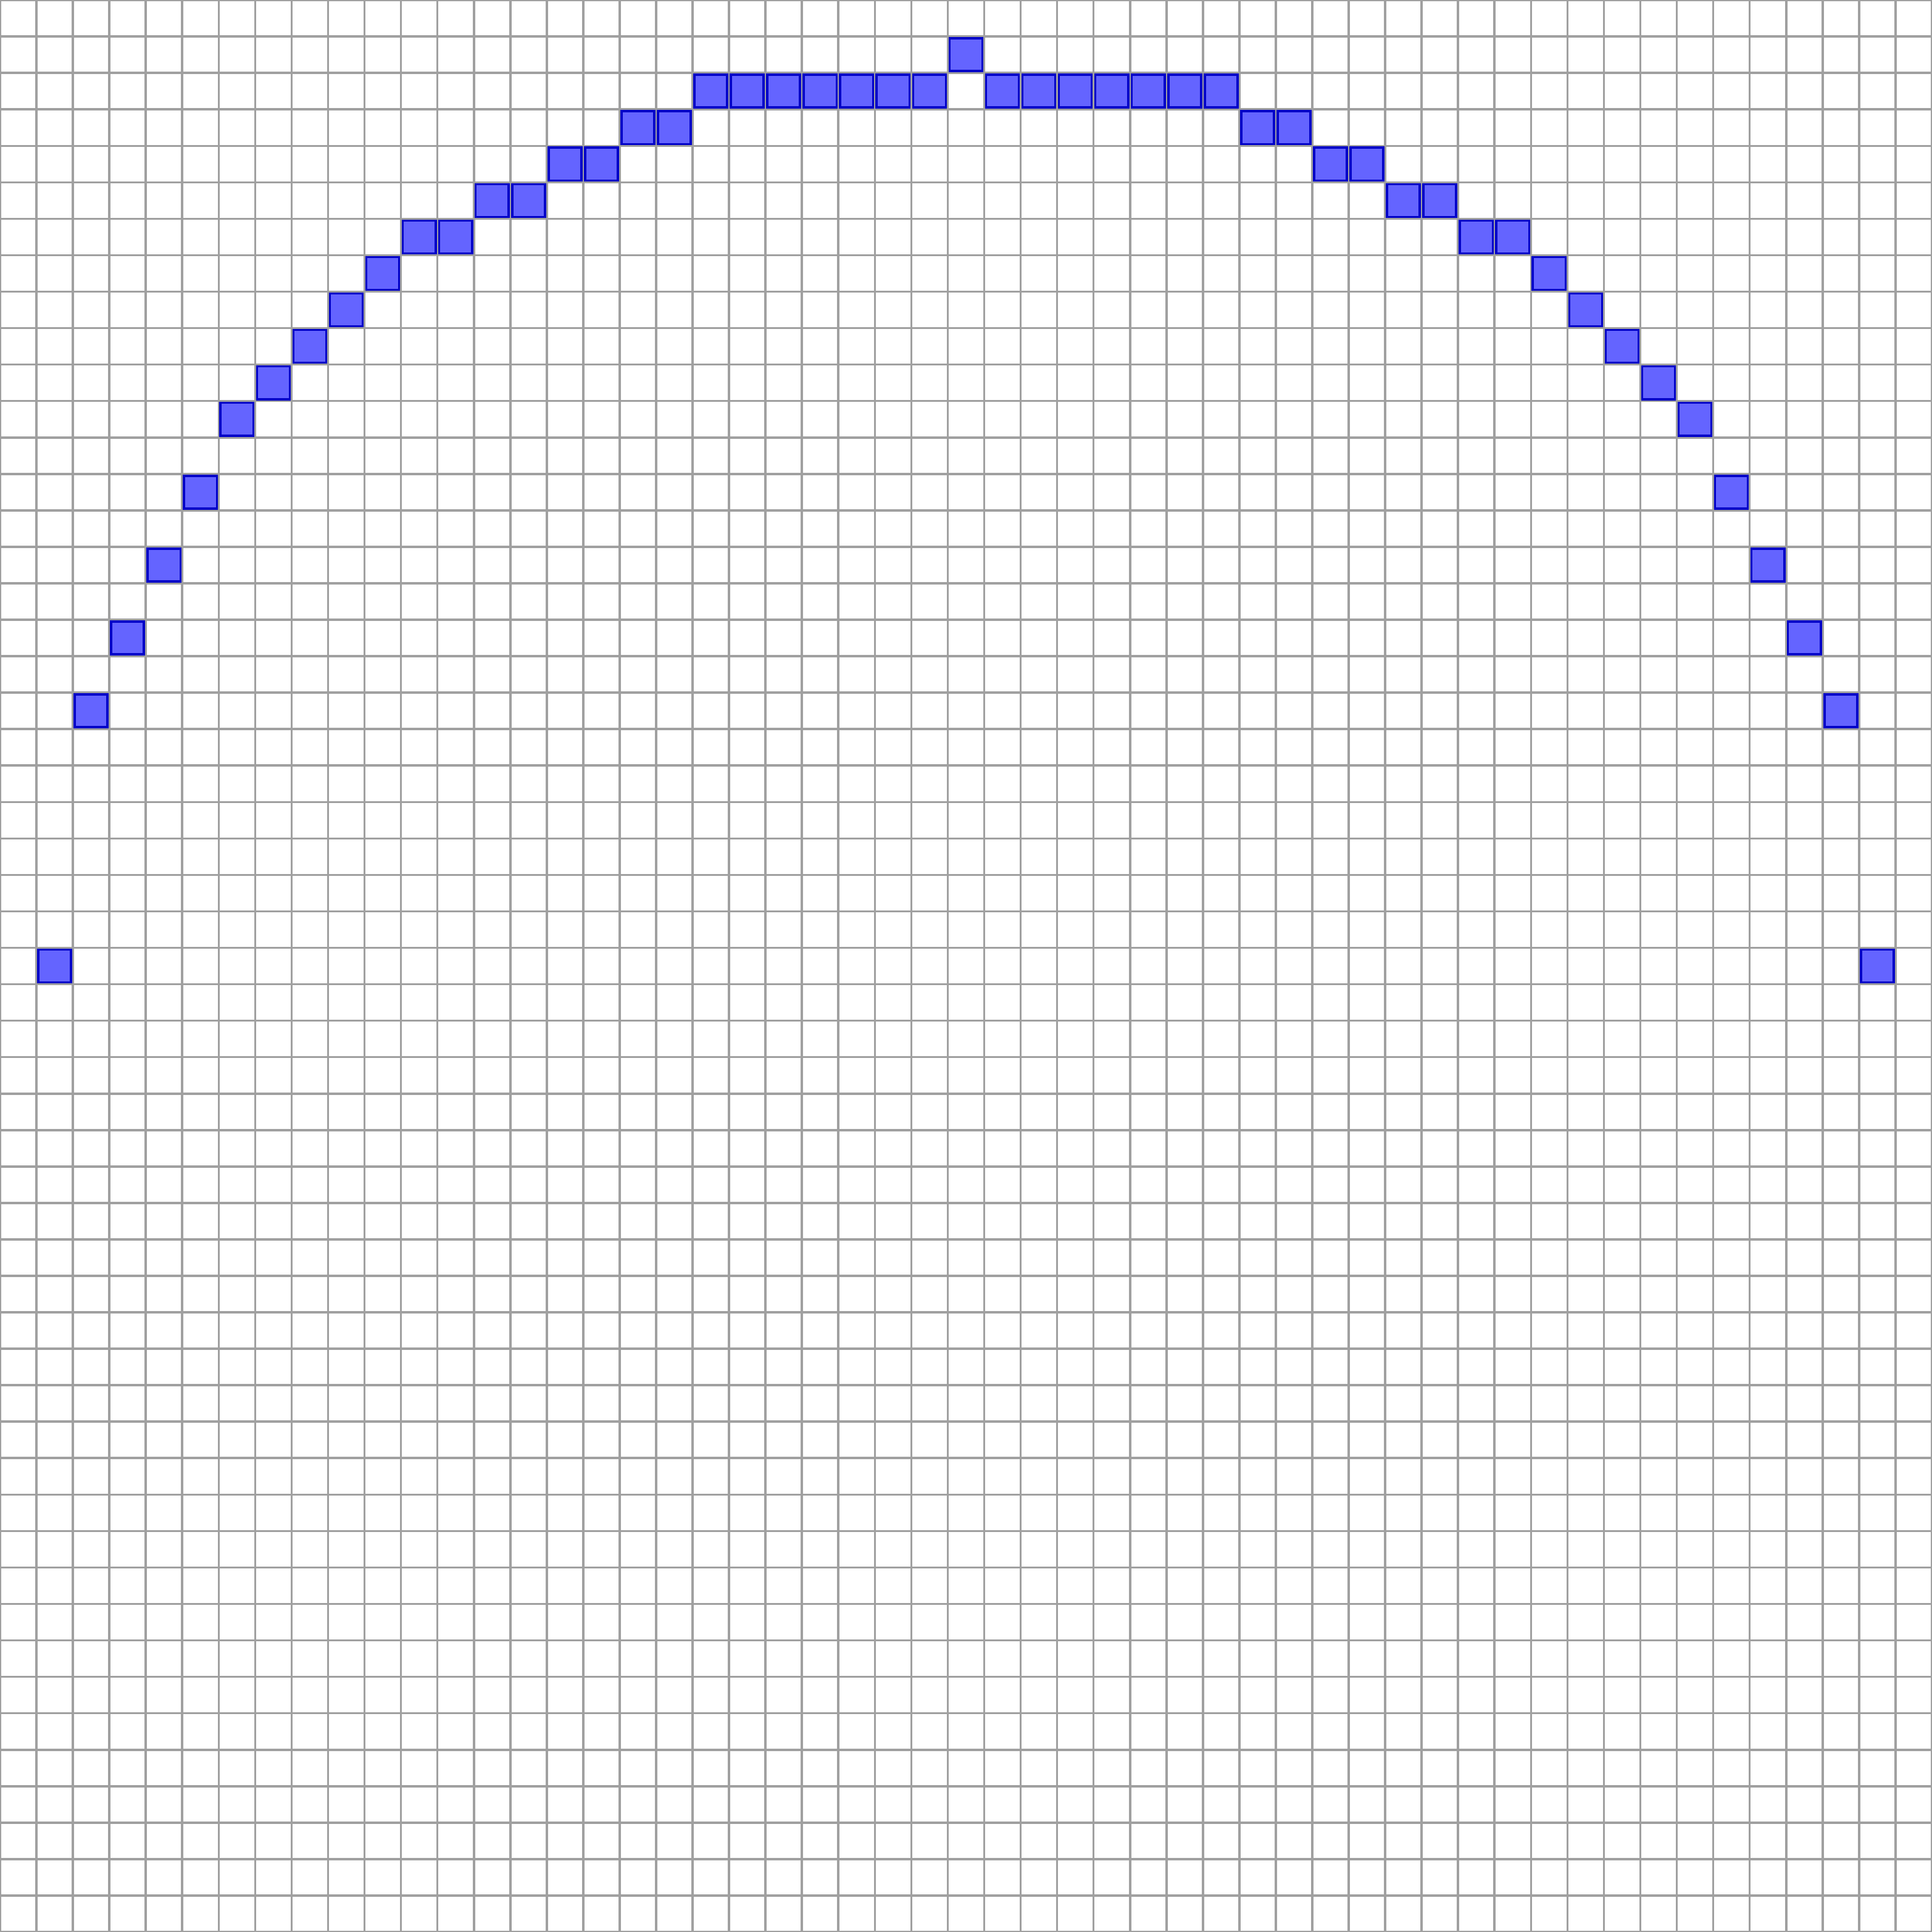
\includegraphics[width=2.5cm]{images/digitalSnow/testIntegralInvariantCurvatureEstimator-PartialMask1}
  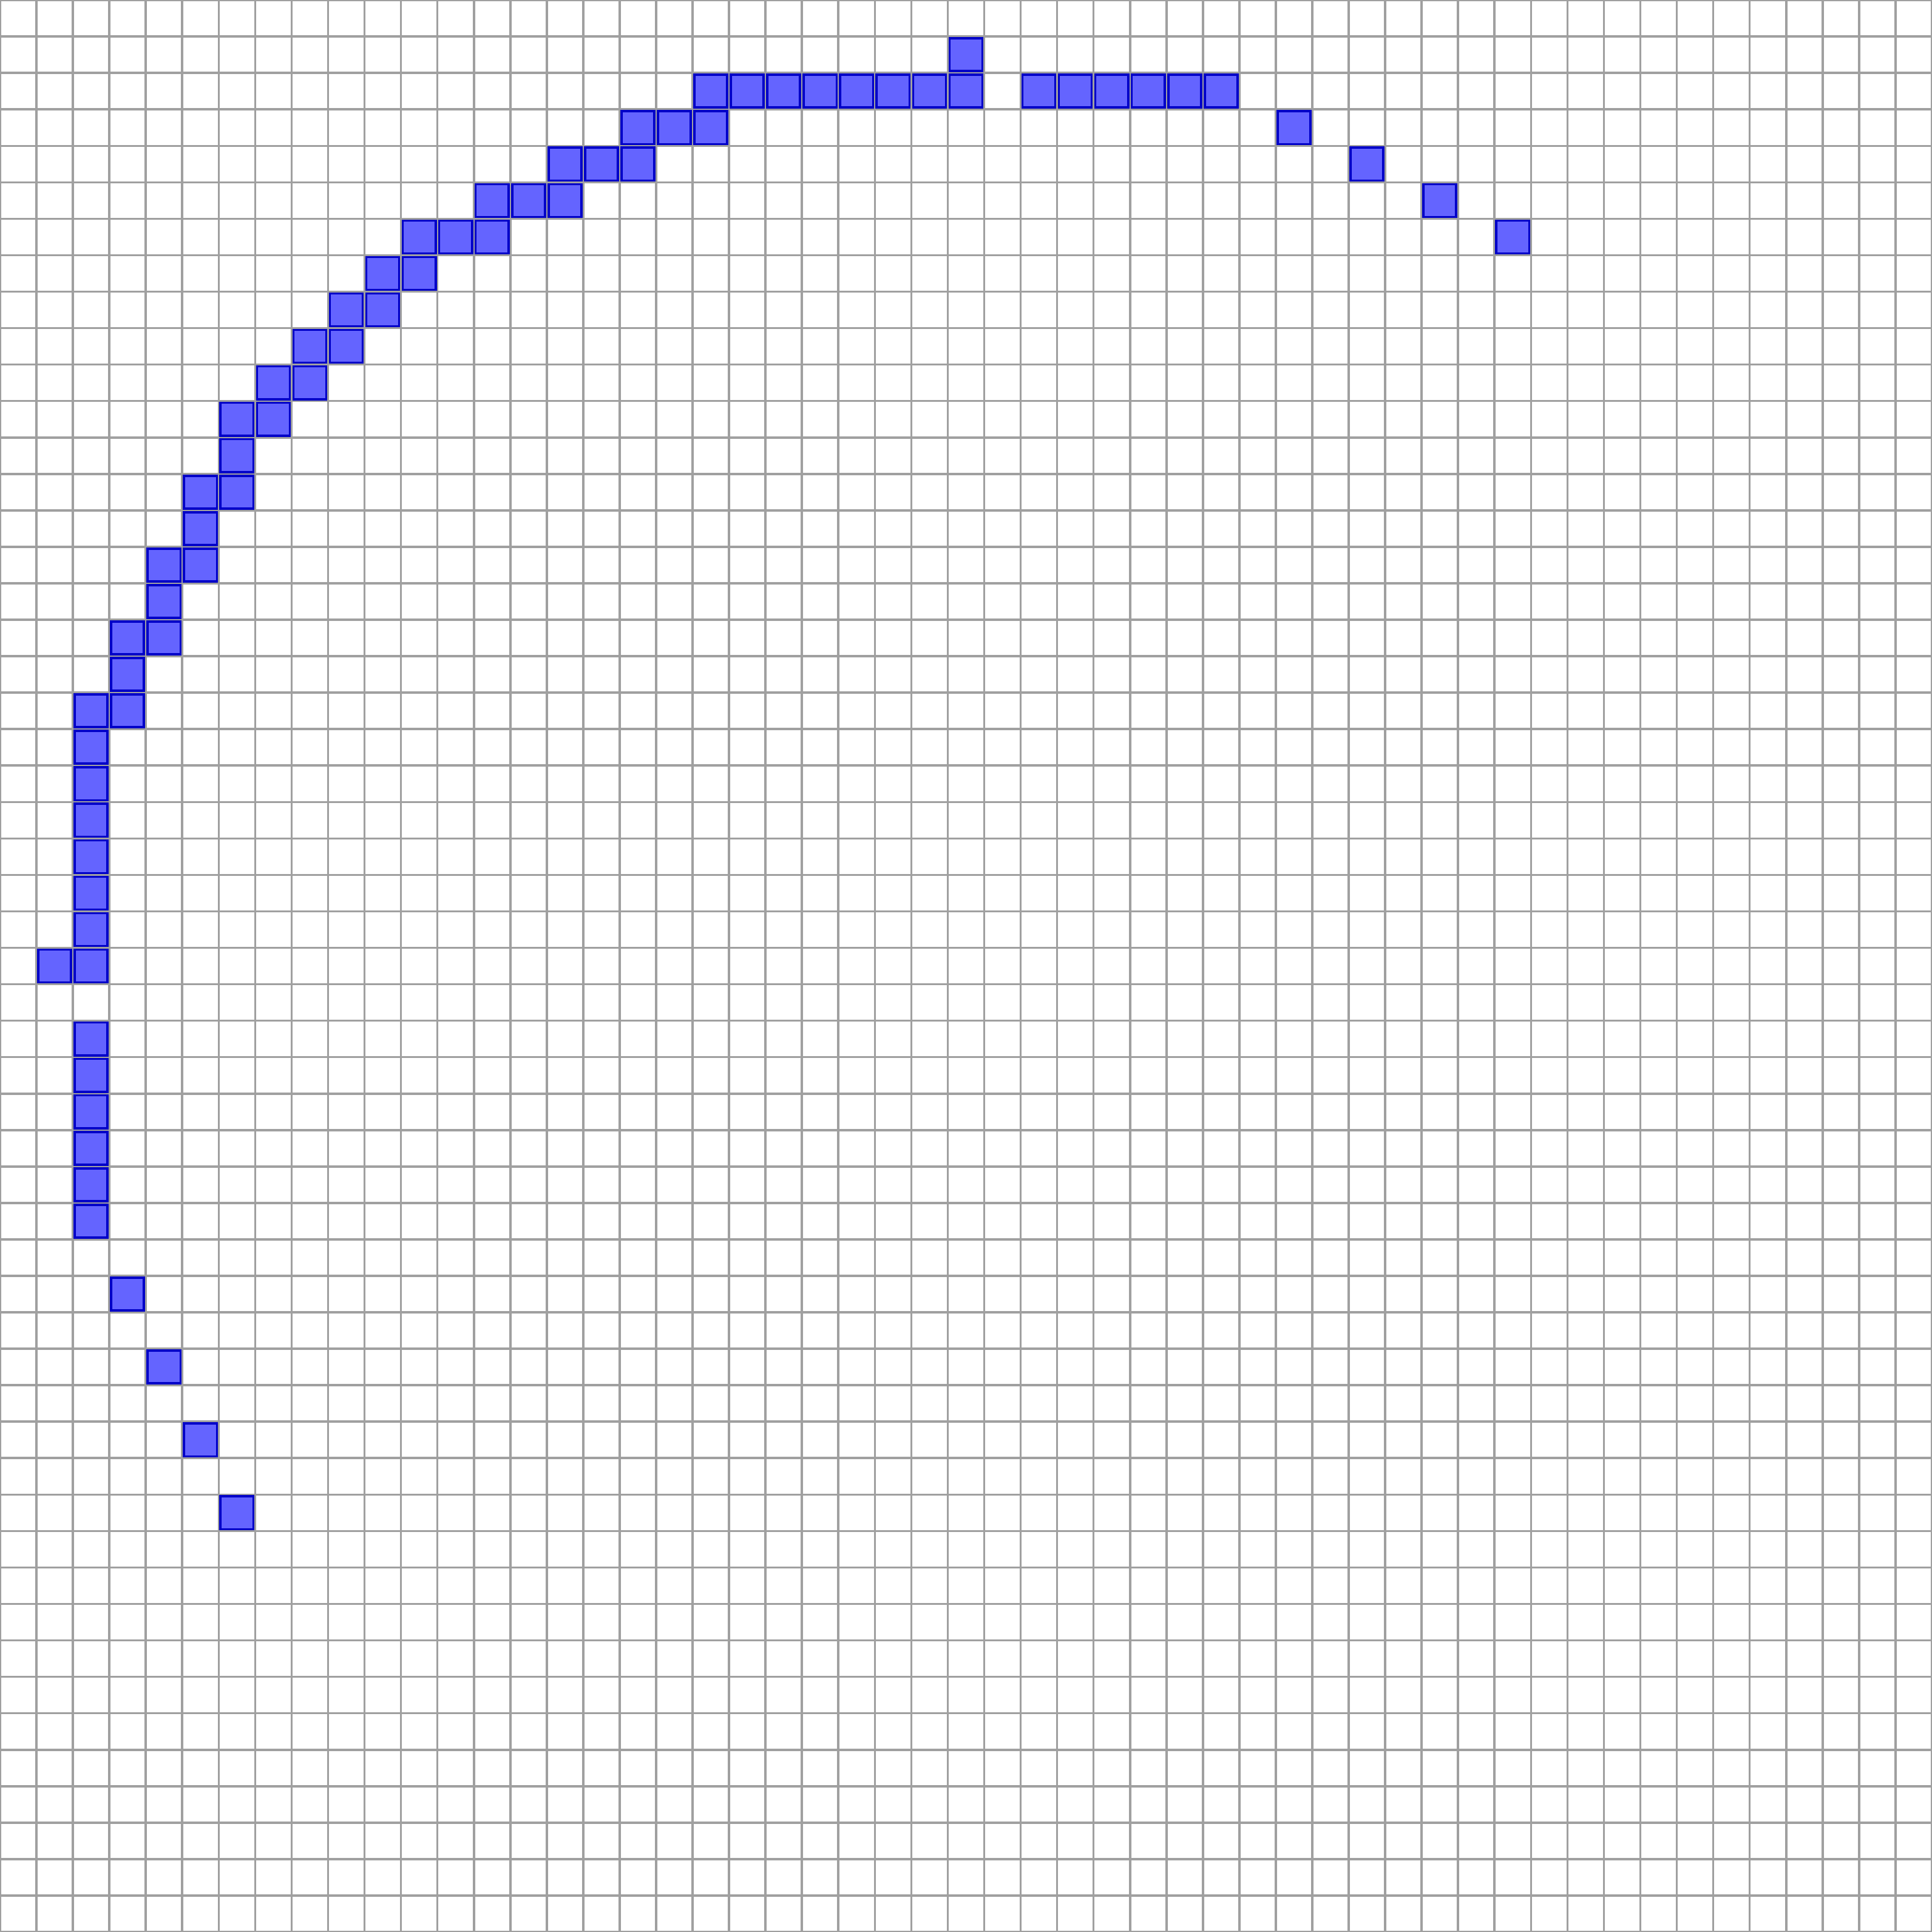
\includegraphics[width=2.5cm]{images/digitalSnow/testIntegralInvariantCurvatureEstimator-PartialMask2}
  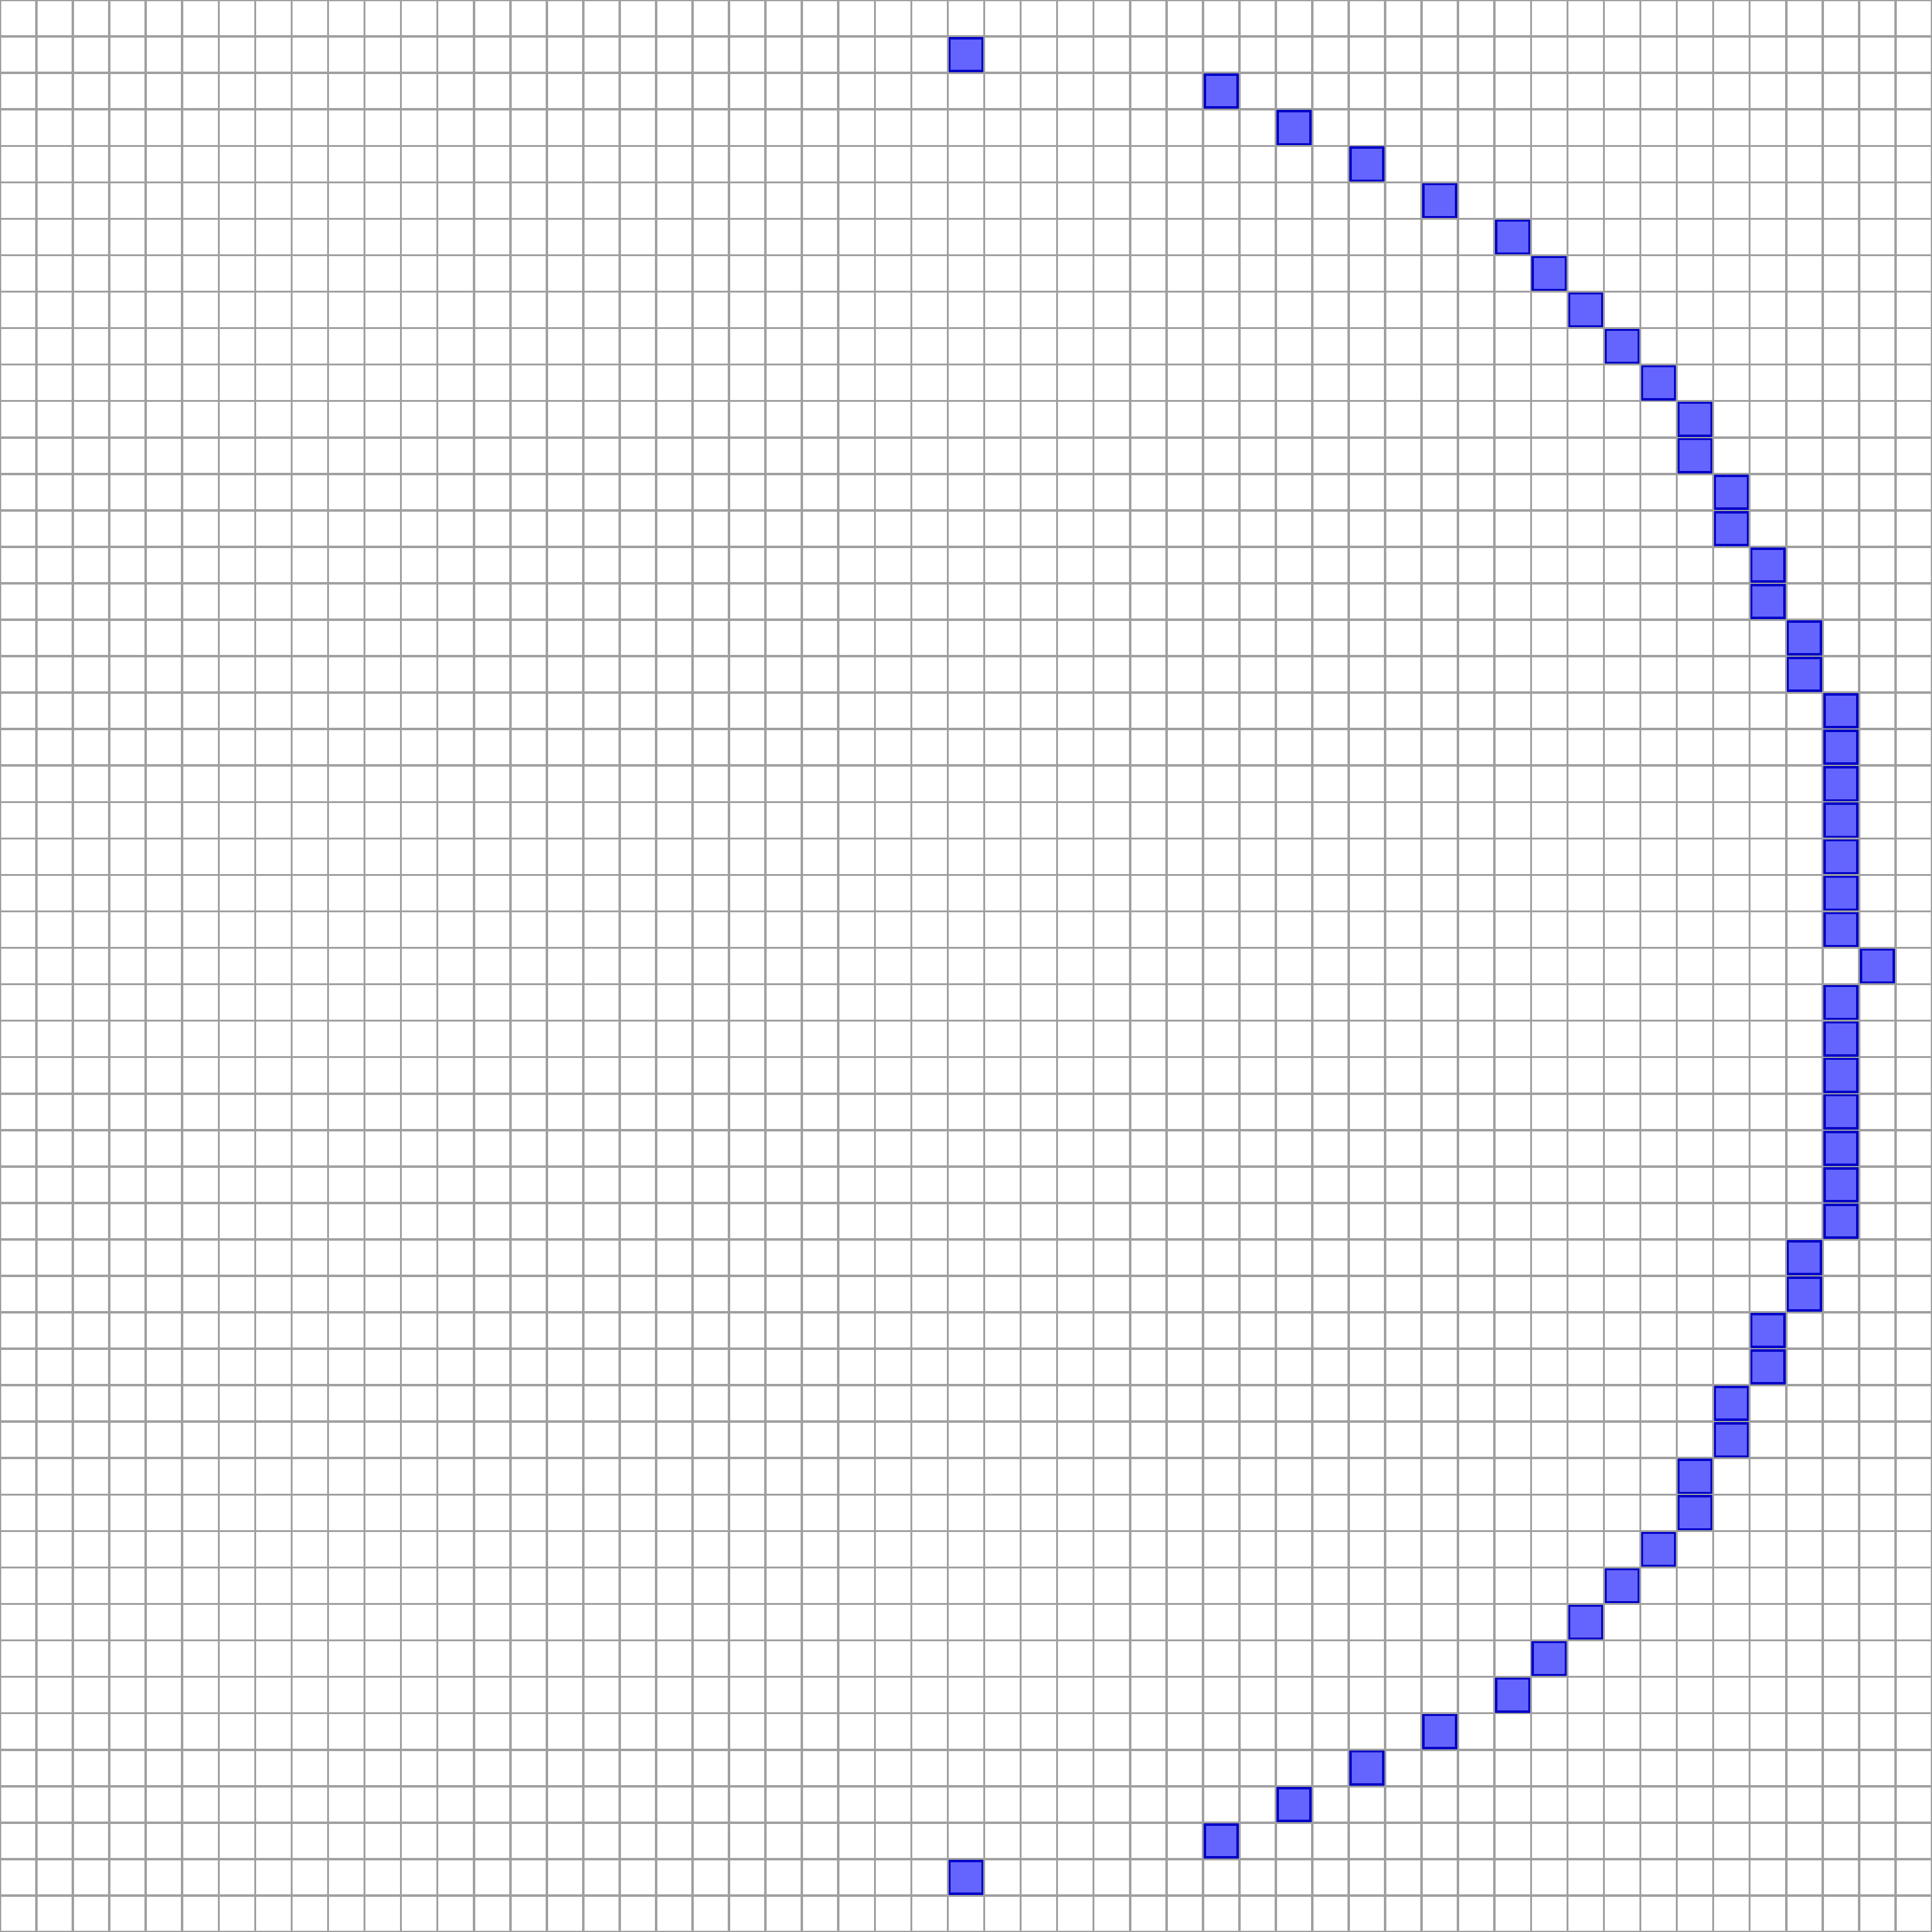
\includegraphics[width=2.5cm]{images/digitalSnow/testIntegralInvariantCurvatureEstimator-PartialMask3}}

  \centerline{
\includegraphics[width=0.1cm,keepaspectratio=false]{images/misc/TransparentPixel}
  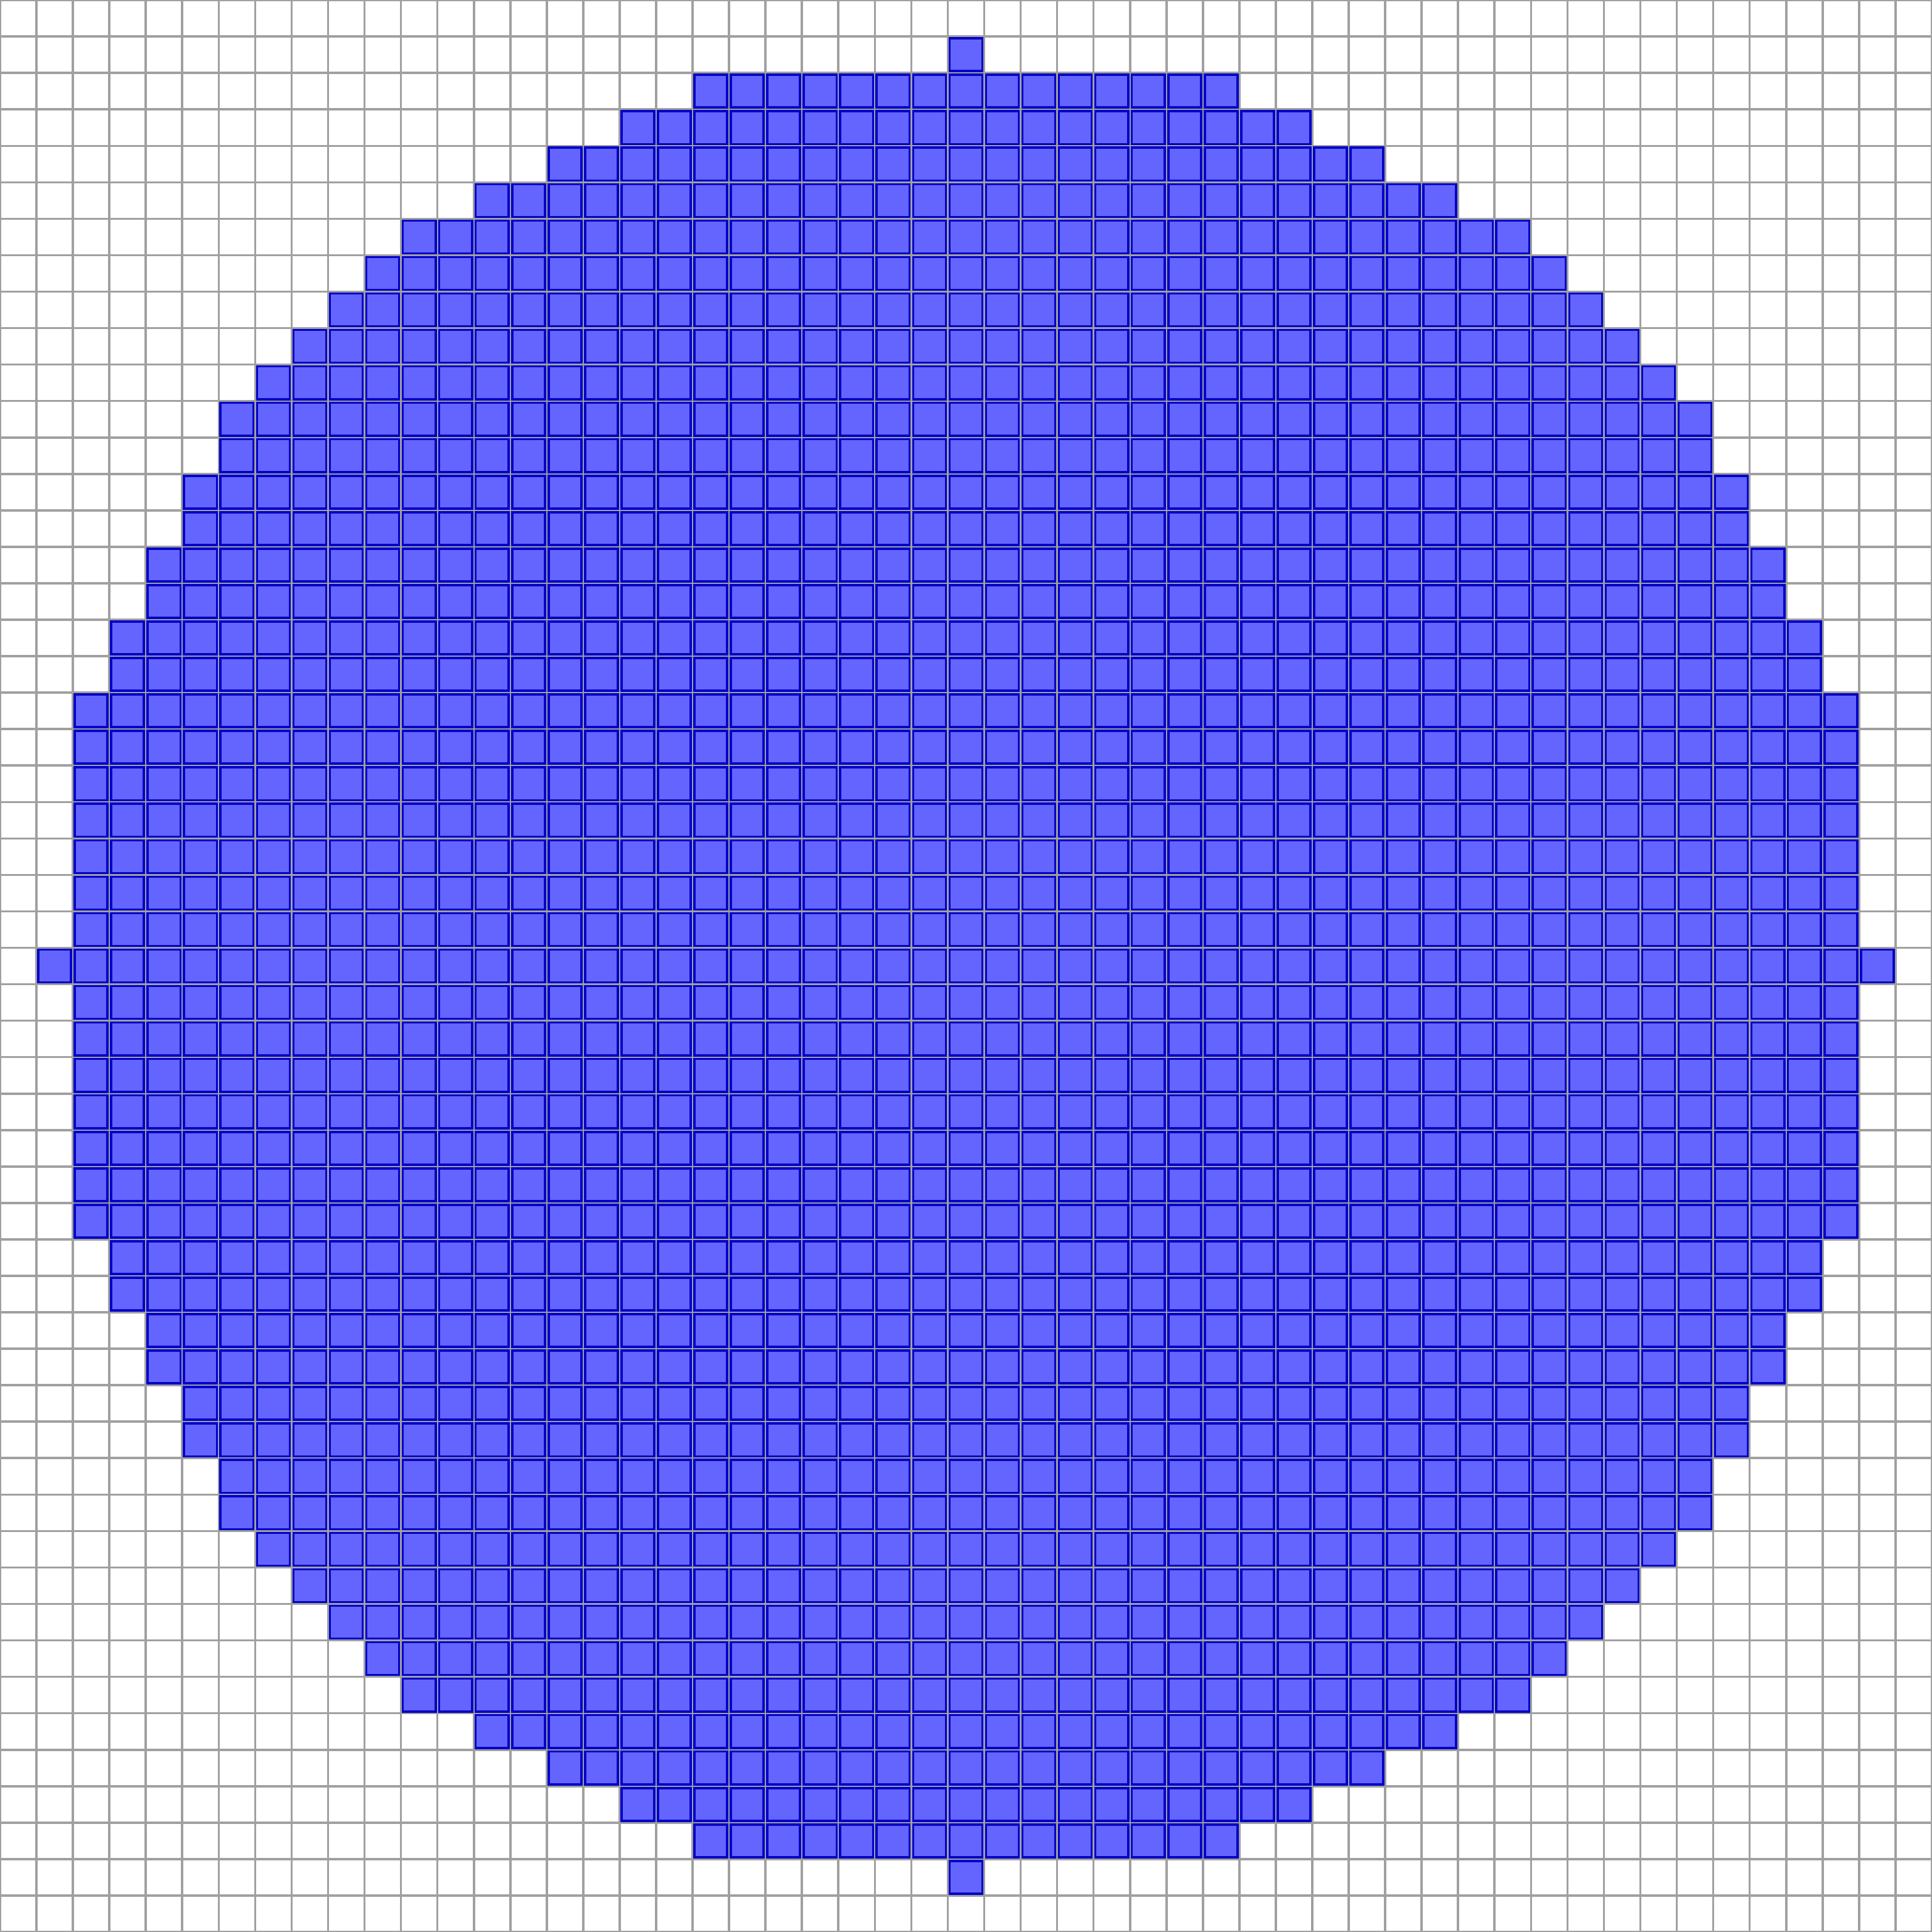
\includegraphics[width=2.5cm]{images/digitalSnow/testIntegralInvariantCurvatureEstimator-PartialMask4}
  
\includegraphics[width=0.17cm,keepaspectratio=false]{images/misc/TransparentPixel}
  
\includegraphics[width=0.3cm,keepaspectratio=false]{images/misc/TransparentPixel}
  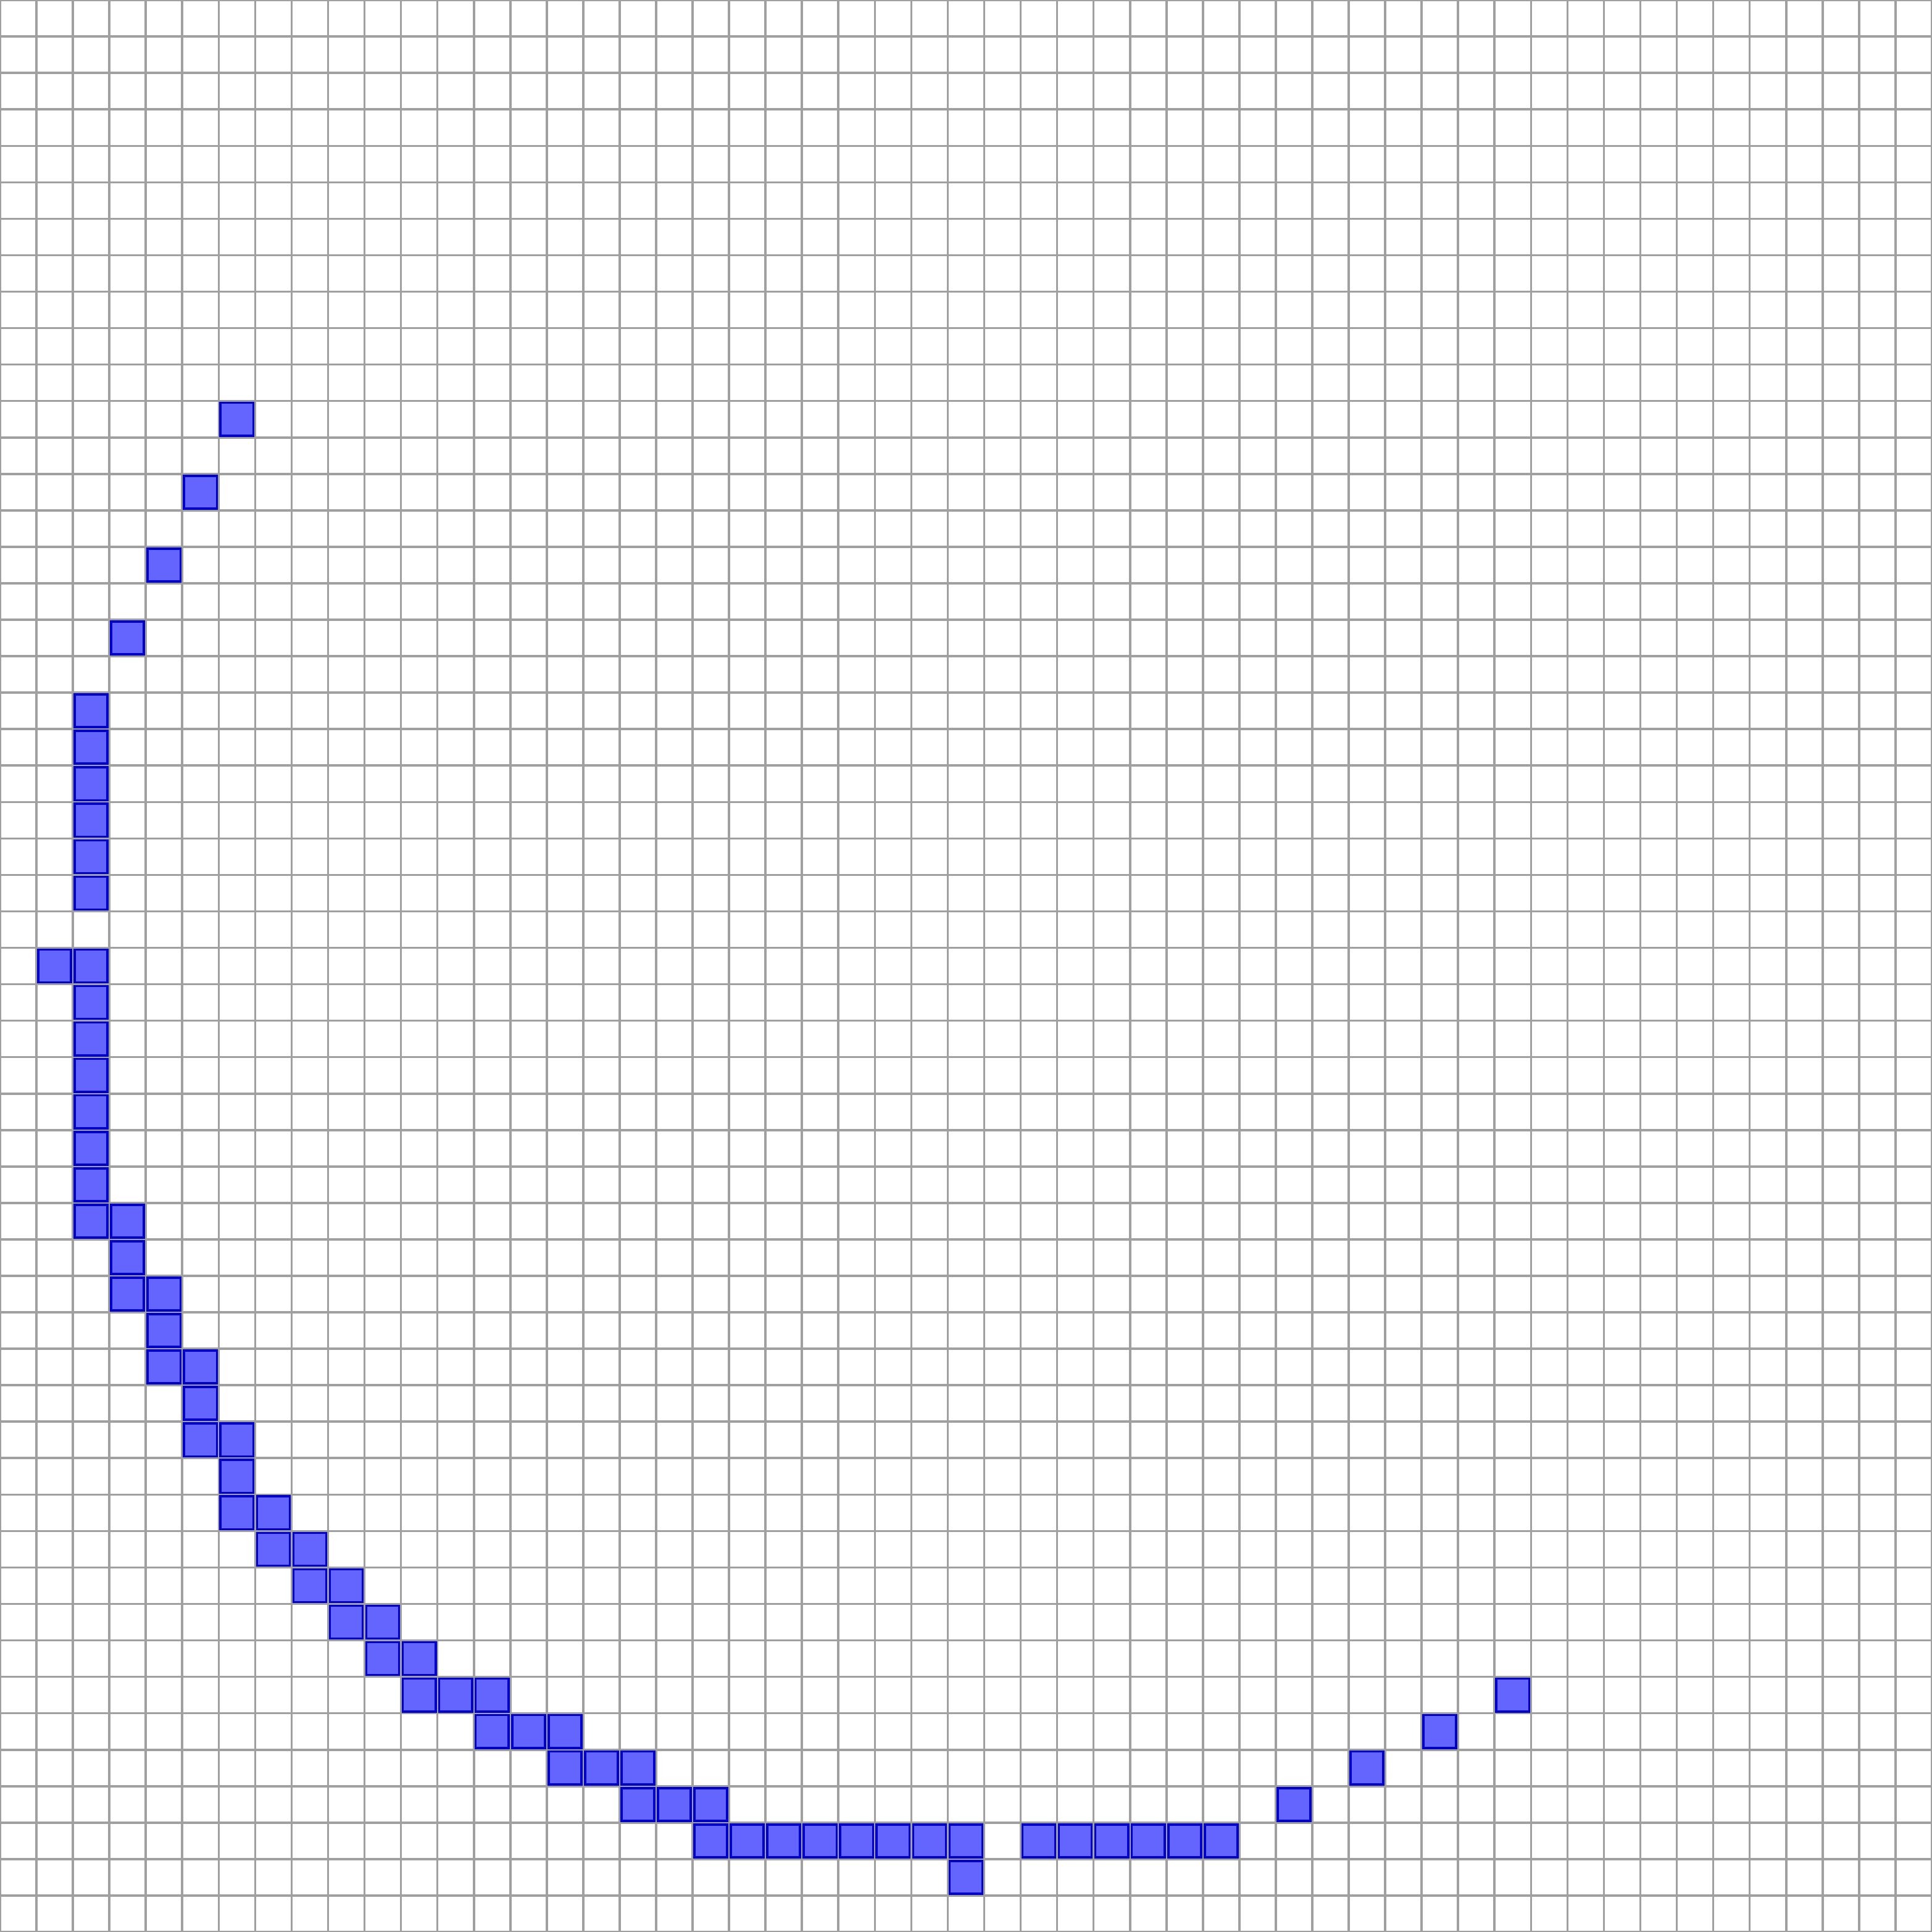
\includegraphics[width=2.5cm]{images/digitalSnow/testIntegralInvariantCurvatureEstimator-PartialMask8}
  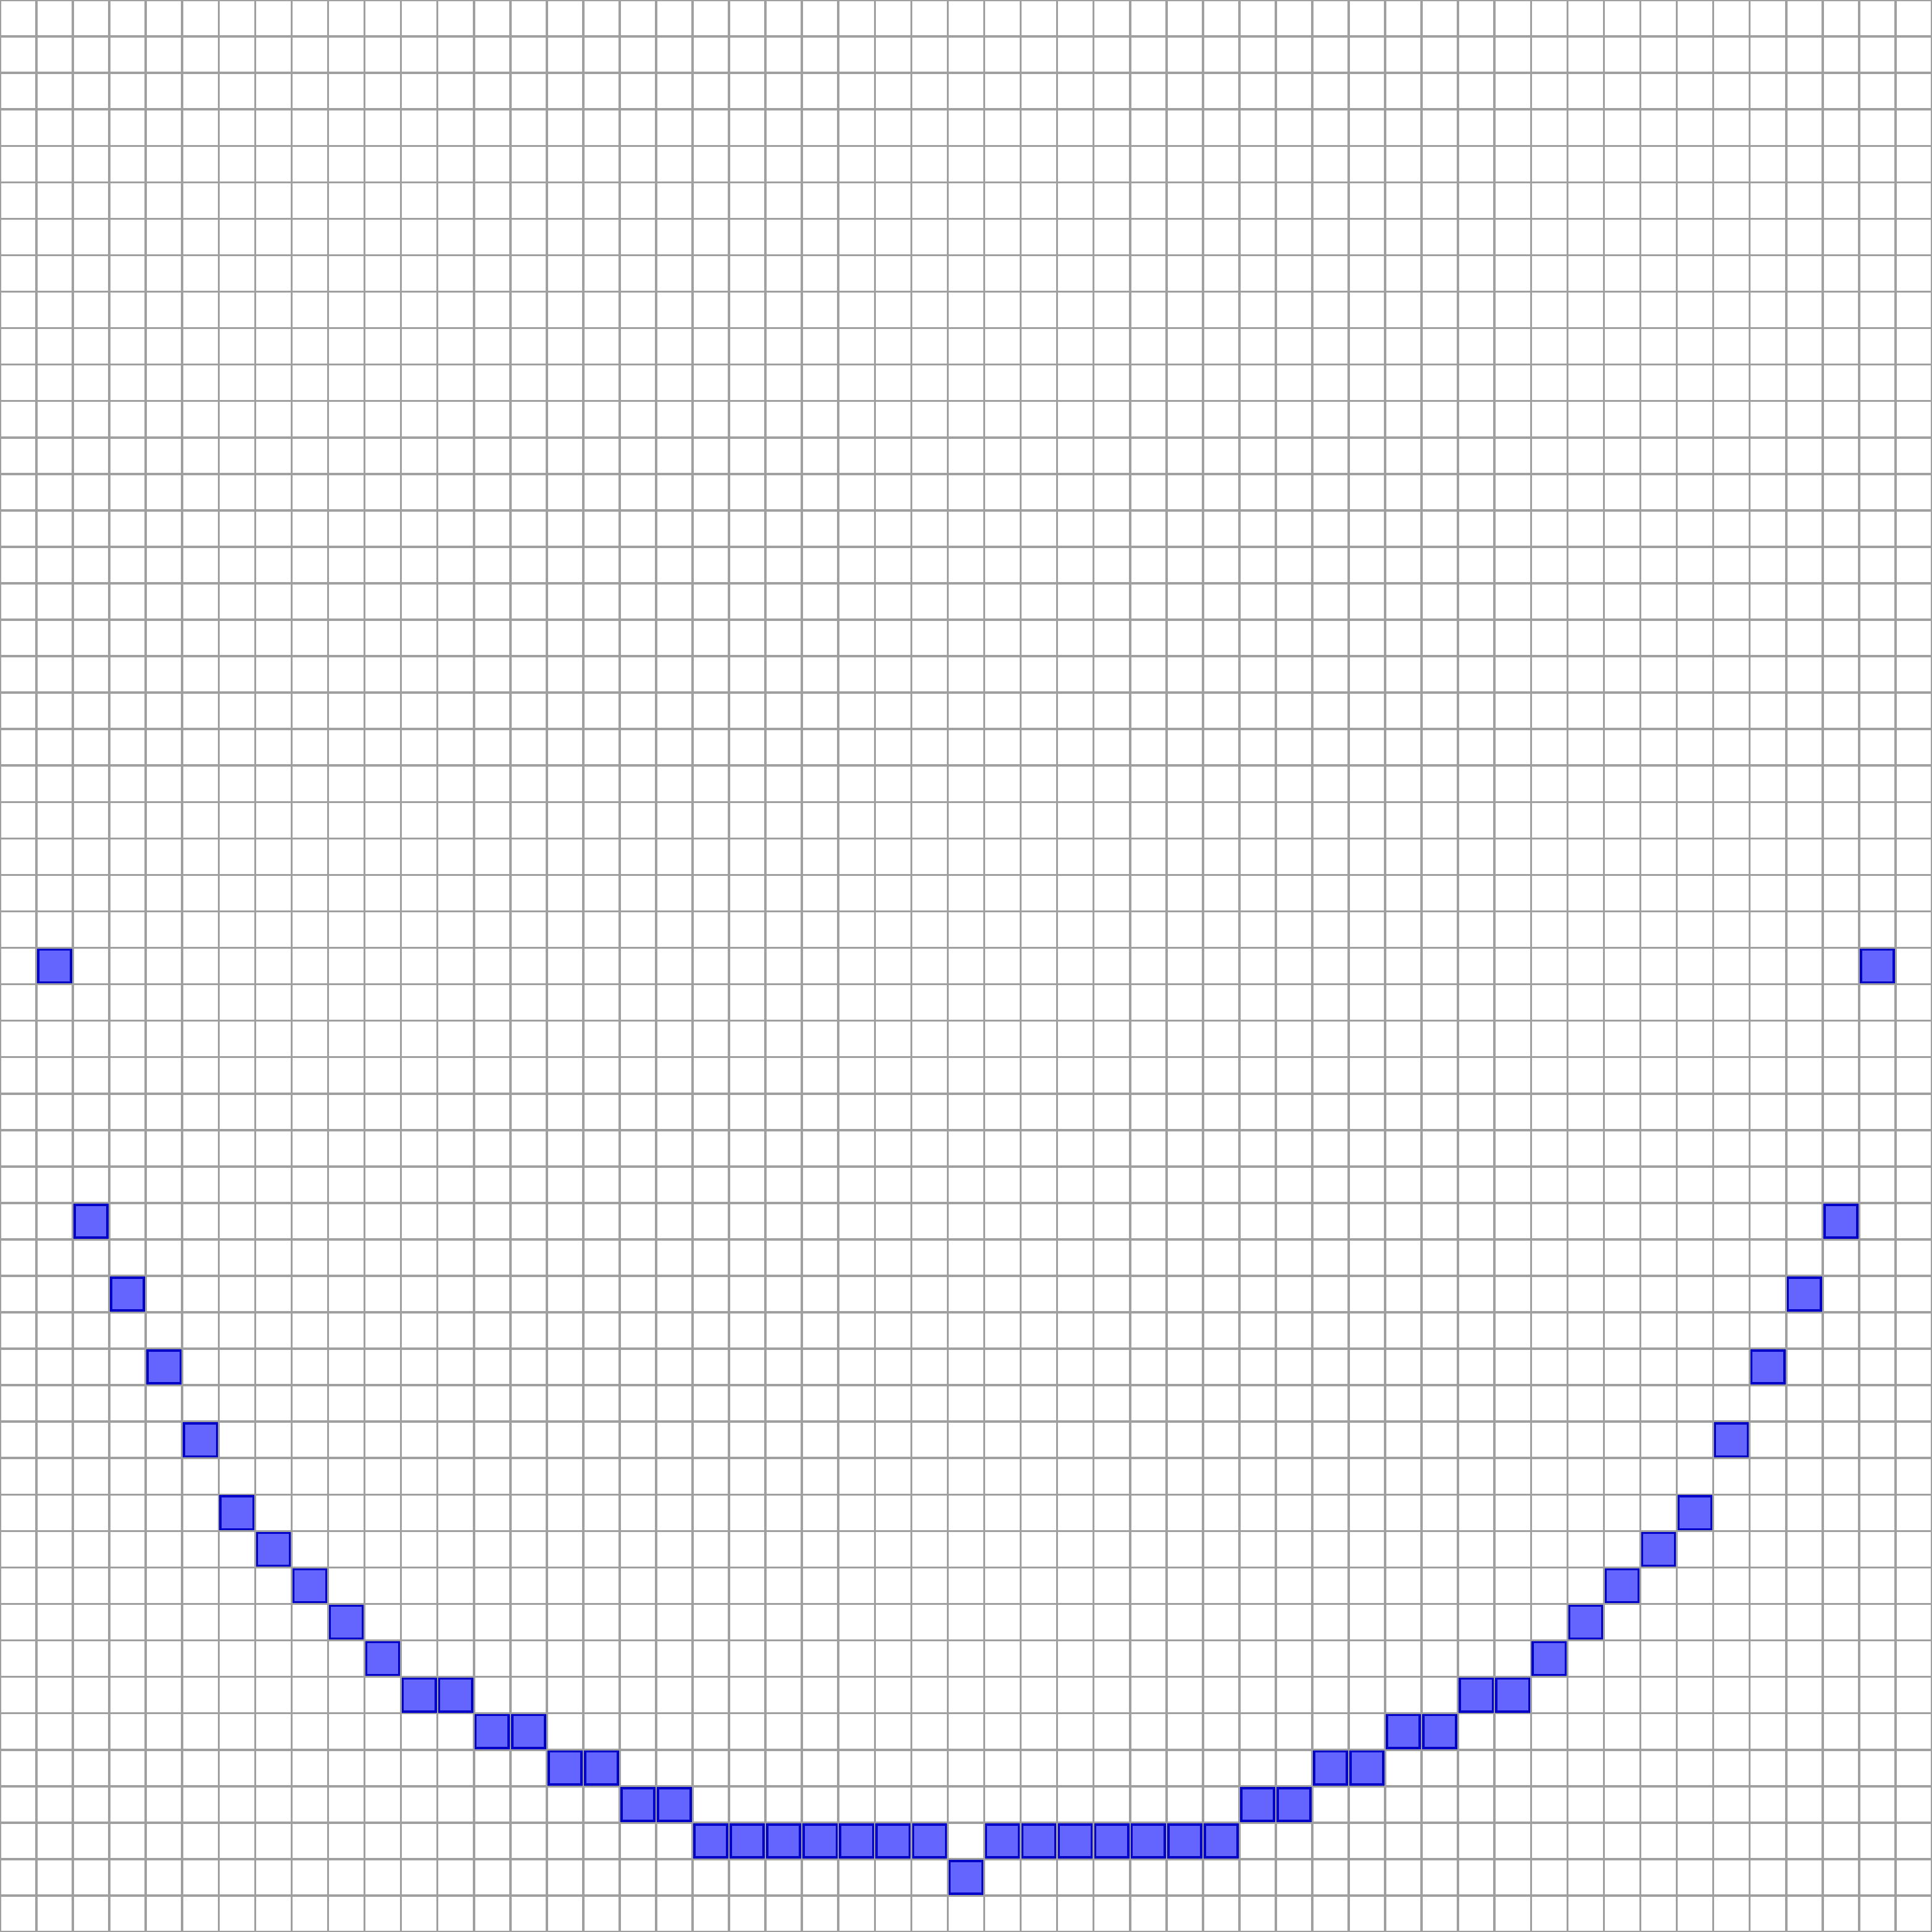
\includegraphics[width=2.5cm]{images/digitalSnow/testIntegralInvariantCurvatureEstimator-PartialMask7}
  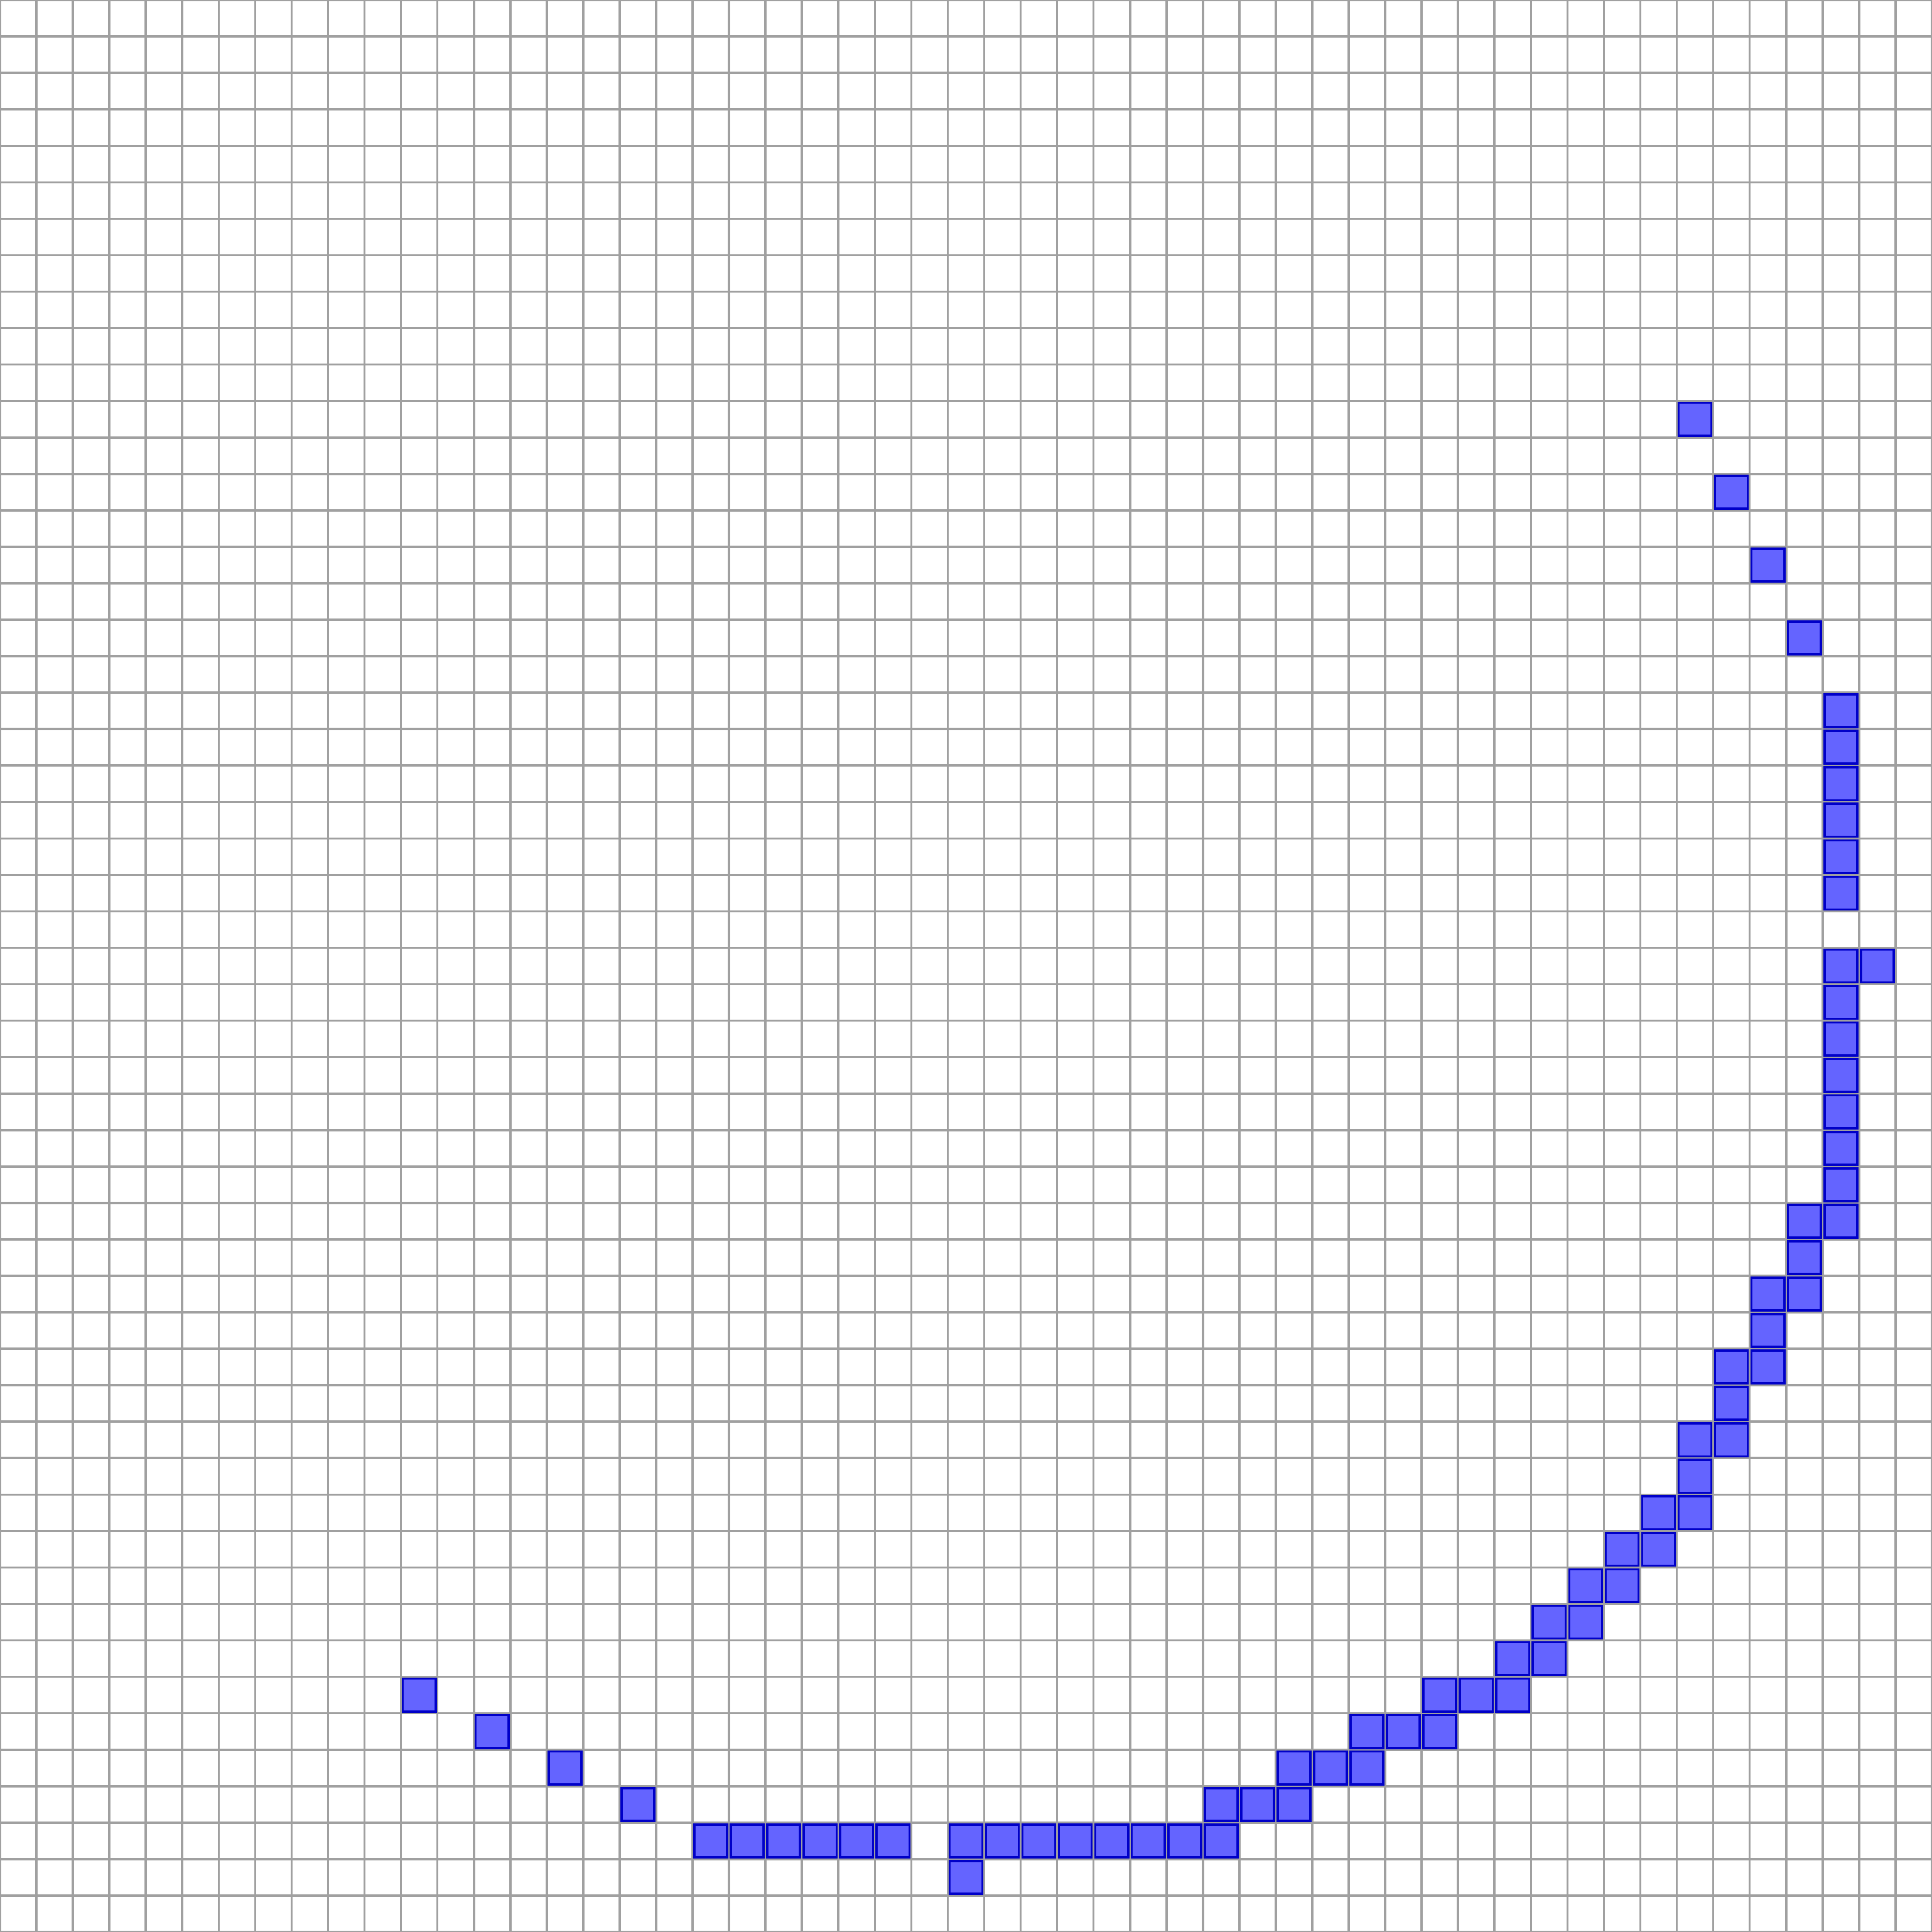
\includegraphics[width=2.5cm]{images/digitalSnow/testIntegralInvariantCurvatureEstimator-PartialMask6}
  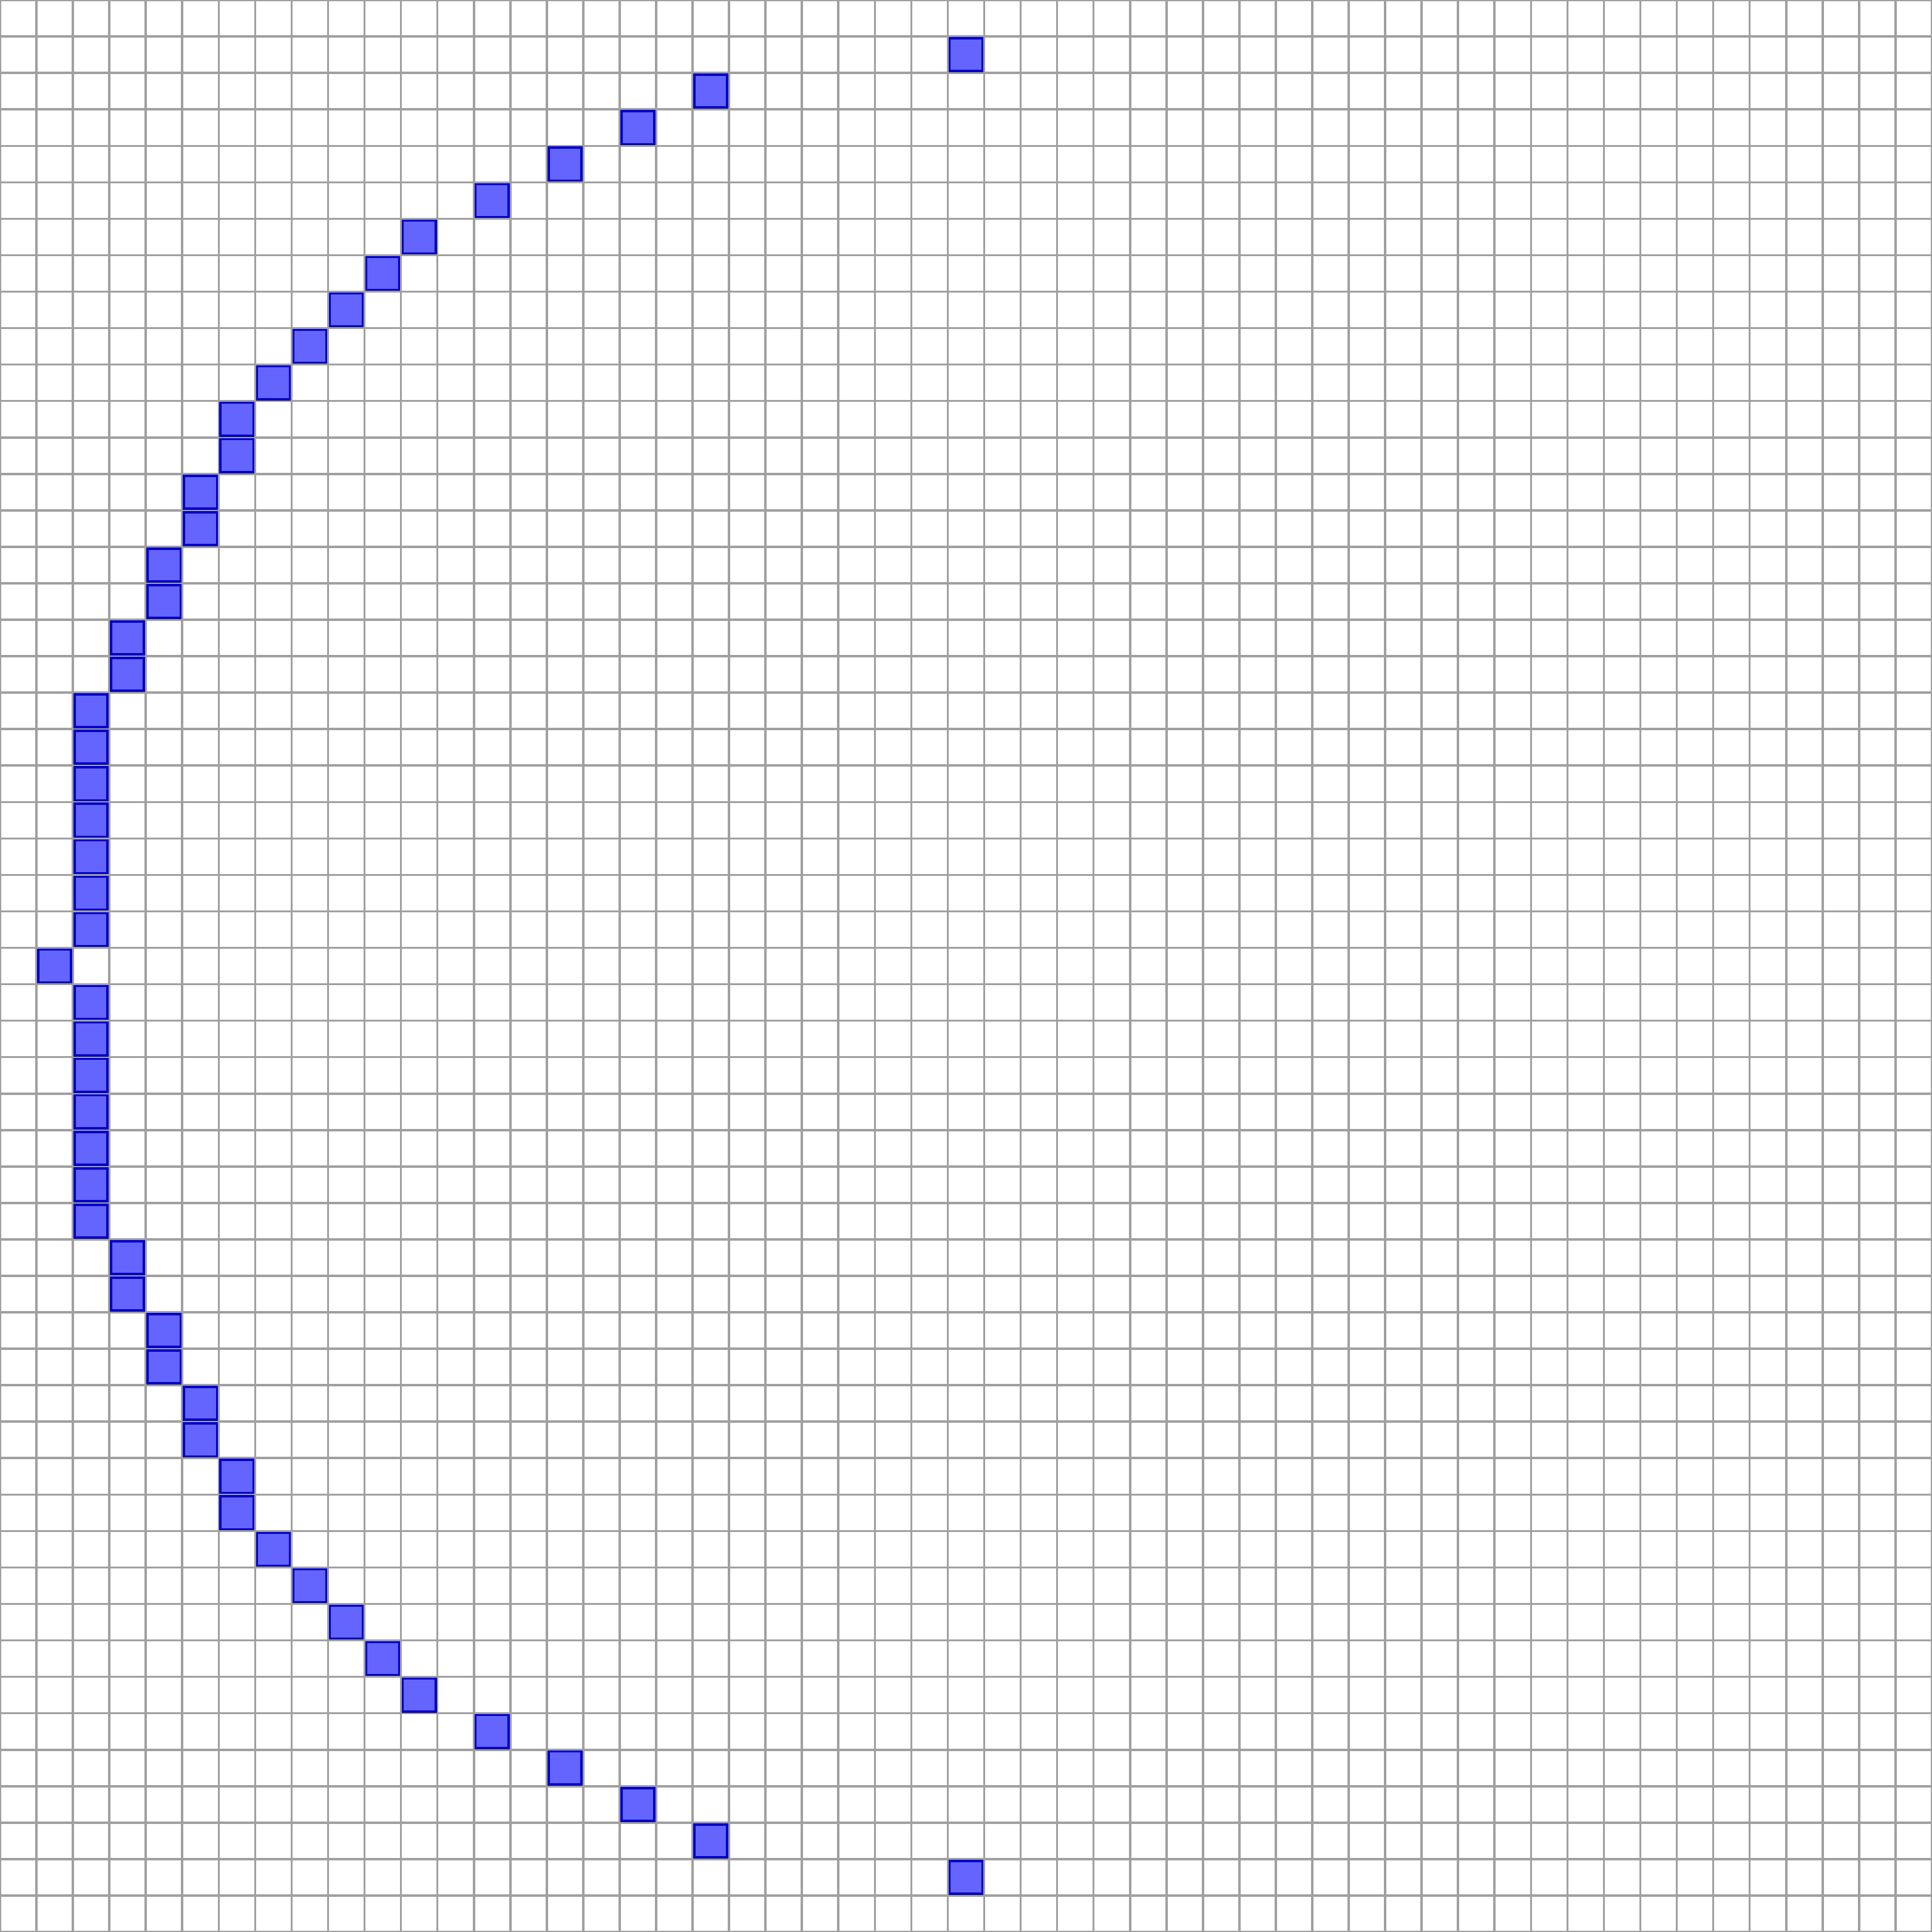
\includegraphics[width=2.5cm]{images/digitalSnow/testIntegralInvariantCurvatureEstimator-PartialMask5}}
  %
  \caption{Illustration de l'optimisation avec les masques partiels de la boule
  2d  pour un pas de discrétisation $h$ donné. \textit{En haut à gauche :}
  Illustration du déplacement du support entier du point $\vx$ au point
  $\vx+\vec{\delta}$, \textit{en bas à gauche :} support 2D entier, \emph{sur la
  droite :} masques partiels de déplacement 0-adjacents.
  \label{fig:MovingKernel2D}}
  %
\end{figure}

Tous les estimateurs de courbure et de singularité conçus pendant cette thèse et
décris dans le \RefChapitre{sec:estimators} et ce chapitre ont été implémentés
dans \DGtal et sont dès à présent disponible librement. Tous les résultats
exposés dans ce document sont reproductibles directement avec les outils de
\DGtal. Pour plus d'informations, se référer à la documentation de
\DGtal\footnote{Documentation du paquet « Géométrie » :
\url{http://liris.cnrs.fr/dgtal/doc/stable/packageGeometry.html}} et à
\cite{Coeurjolly2013Implementation}.
